\documentclass[11pt,reqno]{amsart}

\usepackage[margin=1.0in]{geometry}
\usepackage{amsmath,amssymb,amsthm,mathtools}
\usepackage{booktabs,array}
\usepackage{graphicx}
\usepackage{xcolor}
\usepackage{hyperref}

\definecolor{navy}{HTML}{0F172A}
\definecolor{accent}{HTML}{1B5E7A}
\hypersetup{
  colorlinks=true,
  linkcolor=accent,
  citecolor=accent,
  urlcolor=accent,
  pdftitle={Uncloakable Standing Waves and Prescribed Multi-Attractor Coexistence in Polygonal Sobolev Tanks}
}

\newtheorem{theorem}{Theorem}[section]
\newtheorem{proposition}[theorem]{Proposition}
\newtheorem{lemma}[theorem]{Lemma}
\newtheorem{corollary}[theorem]{Corollary}
\theoremstyle{definition}
\newtheorem{definition}[theorem]{Definition}
\theoremstyle{remark}
\newtheorem{remark}[theorem]{Remark}

\newcommand{\R}{\mathbb{R}}
\newcommand{\C}{\mathbb{C}}
\newcommand{\Z}{\mathbb{Z}}
\newcommand{\N}{\mathbb{N}}
\newcommand{\Q}{\mathbb{Q}}
\DeclareMathOperator{\Fix}{Fix}
\DeclareMathOperator{\diam}{diam}
\DeclareMathOperator{\rank}{rank}
\DeclareMathOperator{\Id}{Id}

\title[Uncloakable Standing Waves and Multi-Attractor Coexistence]{Uncloakable Standing Waves and Prescribed\\
Multi-Attractor Coexistence in Polygonal Sobolev Tanks}

\author{Project ReMath}
\date{November 24, 2026}
\subjclass[2020]{Primary 35P05, 37E10, 76U05; Secondary 35L20, 37C83, 47A75}
\keywords{Sobolev equation, internal wave attractors, chess billiards, boundary circle homeomorphism, Dirichlet eigenfunctions, coexistence, prescribed Lyapunov exponents, Lean~4 formalization}

\setlength{\emergencystretch}{1.2em}
\begin{document}

\begin{abstract}
Motivated by the classical Soviet school of S.~L.~Sobolev (1954), R.~A.~Aleksandryan (1949/1960), T.~I.~Zelenyak (1965/1970), and M.~V.~Fokin (1994--2002) on small oscillations of a rotating or stratified inviscid fluid in bounded domains, we study the Dirichlet streamfunction operator $T = \Delta_D^{-1}\partial_z^2$ on $H_0^1(\Omega)$ (intertwined via $P\Delta_D = \Delta_D T$ with $P = \partial_z^2 \Delta_D^{-1}$ on $H^{-1}(\Omega)$) inside bounded convex polygonal tanks $\Omega \subset \R^2$, alongside a companion translation-surface analysis of nonconvex orthogonal domains. On any convex polygon at interior spectral parameter $E = \lambda^2 \in (0,1)$, the stationary equation $(1-\lambda^2)u_{zz} - \lambda^2 u_{xx} = 0$, $u|_{\partial\Omega} = 0$, is hyperbolic with fixed characteristic ray slopes $\pm s$, $s = \tan\theta = \sqrt{1-\lambda^2}/\lambda$, and reduces via Aleksandryan's boundary reflection map $b_\lambda = \gamma_\lambda^+\gamma_\lambda^-$ to an orientation-preserving piecewise-affine circle homeomorphism.

First, we establish the complete finite-energy $H_0^1(\Omega)$ boundary-profile criterion on arbitrary convex polygons, including endpoint geometric-shell energy scaling at common extrema and constancy along characteristic edges. This yields a bounding-box common-extremum annihilation theorem showing $\sigma_p(T) = \varnothing$ for every triangle (uniformly across all characteristic angles) and every axis-diagonal diamond, as well as a translation-surface spectral theorem for nonconvex orthogonal polyominoes (showing that every $a\times b$ rectangular-grid polyomino shares the exact point spectrum of the $a\times b$ mesh rectangle---matching the unit square iff $a/b \in \Q$---while separated sine products are incomplete in $H_0^1$ on the L-triomino).

Second, we prove the \emph{Universal Half-Amplitude Uncloakability Theorem}: on any convex polygon at a noncharacteristic frequency with rational rotation, every finite-energy standing mode $u \in H_0^1(\Omega)$ satisfies $\|u\|_{L^\infty(\Gamma)} = \max_{w \in H(\partial\Omega)} |w - c_\Gamma| \ge \frac{1}{2}\|u\|_{L^\infty(\Omega)}$ along the spatial path $\Gamma$ of \emph{every} coexisting regular periodic ray (including every attracting wave-attractor circuit), with sharp constant $1/2$. Thus no standing wave can be spatially cloaked from a coexisting wave attractor.

Third, we establish geometric bounds and inverse-design theorems for multi-attractor coexistence. On a convex $k$-gon at a transverse frequency, the number $m$ of two-sided attracting cycles across all periods obeys $m \le k-3$ (attained by polygons with rational vertices and by every odd regular $N$-gon with no characteristic edge at $\lambda = 1/\sqrt{2}$). Requiring a coexisting neutral standing-wave beam forces the universal upper bound $m \le k-4$ at arbitrary period---excluding mixed dynamics in all convex quadrilaterals---and sharp, attained period-two ceilings $m \le \max(0, k-5)$ (minimal period-two coexistence at $k=6$) and $m \le \max(0, h-3)$ under central symmetry ($2h \ge 8$ minimal). Conversely, for every $m \ge 1$, prescribed heights $0 < r_1 < \dots < r_m < a < 1$, and prescribed contraction factors $0 < \kappa_i < 1$, we construct explicit convex $(m+5)$-gons and centrally symmetric $(2m+6)$-gons realizing all $m$ attractors simultaneously while keeping the full infinite-dimensional eigenspace and its Dirichlet energy $4\int_a^1 |h'|^2\,dy$ fixed. A one-parameter pivoting-wall hexagon family exhibits Hausdorff convergence accompanied by an infinite-rank norm-one spectral projection jump $\|\Pi_1 - \Pi_\kappa\| = 1$, while time-reversal symmetry rules out global exterior capture by any attracting circuit. Core algebraic, minimax, cyclic-gap, envelope, and exact-witness components are machine-verified in standalone Lean~4.36.0 with zero \texttt{sorry}.
\end{abstract}

\maketitle

\section{Introduction}

In 1943, studying the stability of a symmetric spinning top containing a fluid-filled cavity (published in \cite{Sobolev1960}), S.~L.~Sobolev was led to the non-Kowalevski evolution equation
\begin{equation}\label{eq:sobolev-evol}
  \partial_t^2 \Delta u + \partial_z^2 u = 0 \qquad \text{in } \Omega \subset \R^2, \qquad u|_{\partial\Omega} = 0,
\end{equation}
presented to the Moscow Mathematical Society on October~2, 1951 (published in 1952) and developed systematically in his landmark 1954 memoir \cite{Sobolev1954}. The same hyperbolic boundary-value structure governs linear two-dimensional inertial waves in a uniformly rotating fluid (with vertical rotation axis, spatial term $f^2 u_{zz}$, and frequency convention $\lambda = \omega/f = \cos\theta$) and, upon exchanging horizontal and vertical axes (or equivalently replacing the spectral parameter $E = \lambda^2$ by $1 - E$, with spatial term $N^2 u_{xx}$ and $\omega/N = \sin\theta$), linear internal gravity waves in a nonrotating uniformly stratified Boussinesq fluid. Separating time via $u(x,z,t) = e^{i\lambda t} u(x,z)$ leads to the bounded self-adjoint spectral problem
\begin{equation}\label{eq:spectral}
  T u = \lambda^2 u, \qquad T = \Delta_D^{-1} \partial_z^2 \quad \text{on } H_0^1(\Omega),
\end{equation}
equipped with the Dirichlet energy inner product $\langle u, v \rangle_{H_0^1} = \int_\Omega \nabla u \cdot \nabla \bar v \, dx\,dz$. Here $\Delta_D \colon H_0^1(\Omega) \to H^{-1}(\Omega)$ is the Dirichlet Laplacian ($\Delta_D u = \partial_x^2 u + \partial_z^2 u$), which intertwines $T$ with the dual operator $P = \partial_z^2 \Delta_D^{-1}$ on $H^{-1}(\Omega)$ via $P \Delta_D = \Delta_D T$. Consequently $T$ and $P$ are unitarily equivalent and share the exact same spectrum and eigenmultiplicities, with $u \in \ker(T - \lambda^2)$ corresponding to $\Delta_D u \in \ker(P - \lambda^2)$.

For every interior spectral parameter $E = \lambda^2 \in (0,1)$, the stationary PDE takes the hyperbolic form
\begin{equation}\label{eq:stationary}
  (1 - \lambda^2) u_{zz} - \lambda^2 u_{xx} = 0 \quad \text{in } \Omega, \qquad u|_{\partial\Omega} = 0.
\end{equation}
Introducing the positive physical ray slope $s$ and ray inclination angle $\theta \in (0,\pi/2)$ to the horizontal,
\begin{equation}\label{eq:slope-conv}
  s = \tan\theta = \frac{\sqrt{1-\lambda^2}}{\lambda}, \qquad \lambda = \cos\theta, \qquad \xi = z + sx, \qquad \eta = z - sx,
\end{equation}
direct substitution converts \eqref{eq:stationary} into the factored wave equation $u_{\xi\eta} = 0$. Unlike acoustic or quantum billiards, where rays obey Snell's law relative to each wall normal, internal-wave reflection preserves the fixed laboratory inclination $\pm\theta$ determined solely by the frequency $\lambda = \cos\theta$. Thus a sloping wall can compress a parallel beam of characteristics upon reflection, funneling wave energy onto a one-dimensional closed periodic limit cycle---an \emph{internal wave attractor}.

A remarkable historical gulf separates two bodies of literature on \eqref{eq:stationary}. Following F.~John's early study of the hyperbolic Dirichlet problem \cite{John1941}, R.~A.~Aleksandryan (in his 1949 Moscow State University dissertation under Sobolev and his 1960 monograph-length paper \cite{Aleksandryan1960}) reduced \eqref{eq:stationary} on convex domains to the boundary circle homeomorphism
\begin{equation}\label{eq:boundary-map}
  b_\lambda = \gamma_\lambda^+ \circ \gamma_\lambda^- \colon \partial\Omega \to \partial\Omega,
\end{equation}
where $\gamma_\lambda^-$ exchanges endpoints along chords of constant $\eta = z - sx$ (physical slope $+s$) and $\gamma_\lambda^+$ exchanges endpoints along chords of constant $\xi = z + sx$ (physical slope $-s$). Aleksandryan established completeness of polynomial eigenfunctions on the disk \cite[\S 9, Thms.~13--14\,bis]{Aleksandryan1960} and constructed smooth domains arbitrarily close to the disk carrying non-almost-periodic solutions. T.~I.~Zelenyak \cite{Zelenyak1965,Zelenyak1970} and M.~V.~Fokin \cite{Fokin1994,Fokin2001,Fokin2002} extended this Novosibirsk school to qualitative asymptotics, singular continuous spectra, and boundary sensitivity. More than three decades later, L.~R.~M.~Maas and F.-P.~A.~Lam \cite{MaasLam1995} and Maas et al.\ \cite{Maas1997} rediscovered geometric wave attractors in oceanography and observed them experimentally in stratified tanks, triggering a modern microlocal and dynamical-systems renaissance led by Colin de Verdi\`ere and Saint-Raymond \cite{CdVSR2020}, Dyatlov and Zworski \cite{DyatlovZworski2019}, Nogueira and Troubetzkoy \cite{NogueiraTroubetzkoy2020}, Lenci, Bonanno, and Cristadoro \cite{LBC2023}, Dyatlov, Wang, and Zworski \cite{DWZ2025}, and Z.~Li \cite{Li2023,Li2024}.

This paper is the first of two self-contained companion articles excavating and extending the Aleksandryan--Zelenyak polygonal boundary-operator theory. While our companion paper \cite{Paper2} investigates single-parameter tilt catastrophes, microscopic corner shaving, all-polygon rigidity, and the regular $N$-gon circle limit, the present paper answers three fundamental structural questions at a fixed frequency inside general convex (and orthogonal nonconvex) polygons:
\begin{enumerate}
  \item \emph{Exact finite-energy spectral criterion}: Exactly when does \eqref{eq:stationary} admit a nonzero $H_0^1(\Omega)$ streamfunction on a polygon with corners and possible characteristic edges, and which polygons have $\sigma_p(T) = \varnothing$?
  \item \emph{Spatial visibility of coexisting standing waves}: If a polygonal tank supports \emph{both} a smooth standing eigenmode $u \in H_0^1(\Omega)$ and a focusing wave-attractor circuit $\Gamma$ at the same frequency, can the standing mode hide inside a calm pocket with zero (or arbitrarily small) amplitude on $\Gamma$?
  \item \emph{Sharp multiplicity and inverse design}: How many attracting circuits can coexist in a convex $k$-gon---both freely and alongside a standing-wave eigenspace---and can their locations and Lyapunov contraction factors be prescribed independently?
\end{enumerate}

\subsection*{Summary of main results}
Throughout, a convex $k$-gon $K = \overline{\Omega} \subset \R^2$ has nonempty interior and genuine vertices (adjacent collinear edges merged). By convention, every periodic circuit is counted once with its attracting orientation, and a \emph{regular} cycle avoids all vertices and grazing chords.

\begin{itemize}
  \item \textbf{Finite-energy polygonal eigenmodes, obstructions, and polyominoes (Section~\ref{sec:pde})}: Theorem~\ref{thm:h1-criterion} characterizes $\ker(T - \lambda^2)$ on every convex polygon via $H^1(\partial K)$ functions invariant under $\gamma_\lambda^\pm$ and constant along characteristic edges, using an exact geometric-shell energy argument at common extremal vertices. Theorem~\ref{thm:periodic-interval} shows that $\ker(T-\lambda^2) \ne \{0\}$ if and only if $b_\lambda^q|_{\mathcal{C}} = \Id$ on an open interval $\mathcal{C}$ whose full dihedral orbit avoids characteristic edges, always ensuring that $\ker(T-\lambda^2)$ contains an infinite-dimensional subspace of $C^\infty(\overline{\Omega})$ modes. Theorem~\ref{thm:common-extremum} proves that a single shared weak extremum of $\xi,\eta$ annihilates $\ker(T-\lambda^2)$, giving $\sigma_p(T) = \varnothing$ for every triangle (including edge-parallel angles where $b^2 = \Id$ or $b^3 = \Id$) and every axis-diagonal diamond. For nonconvex orthogonal polygons, Theorem~\ref{thm:polyomino} proves density of infinite-multiplicity eigenvalues via Masur's theorem and determines the exact point spectrum of every rectangular-grid polyomino via square-tiled ergodicity, while proving that separated sine products are incomplete in $H_0^1$ on the L-triomino.
  \item \textbf{Universal Half-Amplitude Uncloakability (Section~\ref{sec:uncloakability})}: Theorem~\ref{thm:uncloakable} proves that at any noncharacteristic rational-rotation frequency on a convex polygon, for every $u \in \ker(T-\lambda^2)$ (taking its continuous representative) and every regular periodic circuit $\Gamma$ of period $q \ge 2$,
  \[
    \|u\|_{L^\infty(\Gamma)} = \max_{w \in H(\partial\Omega)} |w - c_\Gamma| \ge \tfrac{1}{2}\|u\|_{L^\infty(\Omega)}, \qquad \|u\|_{L^\infty(\Omega)} = \diam H(\partial\Omega),
  \]
  with equality if and only if $H(\partial\Omega) \subseteq \overline{D}(c_\Gamma, \frac{1}{2}\diam H(\partial\Omega))$ (reducing for real-valued modes to $c_\Gamma = \frac{1}{2}(\min H + \max H)$). The constant $1/2$ is sharp and attained on a hexagon with rational vertices (Figure~\ref{fig:p1-fig1}).
  \item \textbf{Multiplicity Bounds and Regular-Polygon Saturation (Section~\ref{sec:multiplicity})}: Theorem~\ref{thm:k-minus-3} proves $m \le k-3$ for two-sided attracting cycles of arbitrary period on any convex $k$-gon (with separate bounds for attractors and repellers at characteristic edges, where the combined count can reach $4 > 6-3$). Theorem~\ref{thm:mixed-bounds} proves the universal mixed-dynamics upper bound $m \le k-4$ across all periods (ruling out mixed dynamics in all convex quadrilaterals; sharpness for $q \ge 3$ open), together with the sharp period-two ceilings $m \le \max(0, k-5)$ (minimal period-two coexistence at $k=6$) and $m \le \max(0, h-3)$ for centrally symmetric $2h$-gons (minimal $2h=8$; Figure~\ref{fig:p1-fig2}B). Proposition~\ref{prop:odd-regular} proves that every odd regular $N$-gon ($N \ge 5$) with no characteristic edge at $\lambda = 1/\sqrt{2}$ attains $N-3$, and analyzes symmetry-enforced rate pairing and its splitting on the tilted pentagon (Figure~\ref{fig:p1-fig3}A).
  \item \textbf{Prescribed-Rate Inverse Design and Infinite-Rank Spectral Jump (Section~\ref{sec:design})}: Theorem~\ref{thm:hexagon-jump} constructs the minimal period-two coexistence hexagon with rational vertices (contraction $1/2$, exact horizontal-launch basins $(1/4, 1/2, 1/4)$, and universal non-existence of global exterior capture by time reversal) and a one-parameter pivoting-wall family $\Omega_\kappa$ converging in Hausdorff distance to a symmetric neutral tank while the eigenspace projection undergoes an infinite-rank norm-one jump $\|\Pi_1 - \Pi_\kappa\| = 1$. Theorem~\ref{thm:prescribed} realizes arbitrary prescribed heights $0 < r_1 < \dots < r_m < a < 1$ and arbitrary multipliers $0 < \kappa_i < 1$ on sharp convex $(m+5)$-gons and centrally symmetric $(2m+6)$-gons (Figure~\ref{fig:p1-fig2}A) with fixed eigenspace and exact Dirichlet energy $4\int_a^1 |h'|^2\,dy$.
  \item \textbf{Machine-Checked Formalization (Section~\ref{sec:lean})}: Core algebraic, minimax, time-reversal, cyclic-gap, four-chain, central-envelope, prescribed-wall, common-extremum, and exact-witness components are verified in standalone Lean~4.36.0 (\texttt{Uncloakability}, \texttt{MultiplicityBounds}, and \texttt{CornerShavingAndTriangles}) with zero \texttt{sorry} and standard axioms only.
\end{itemize}

\begin{figure}[ht]
\centering
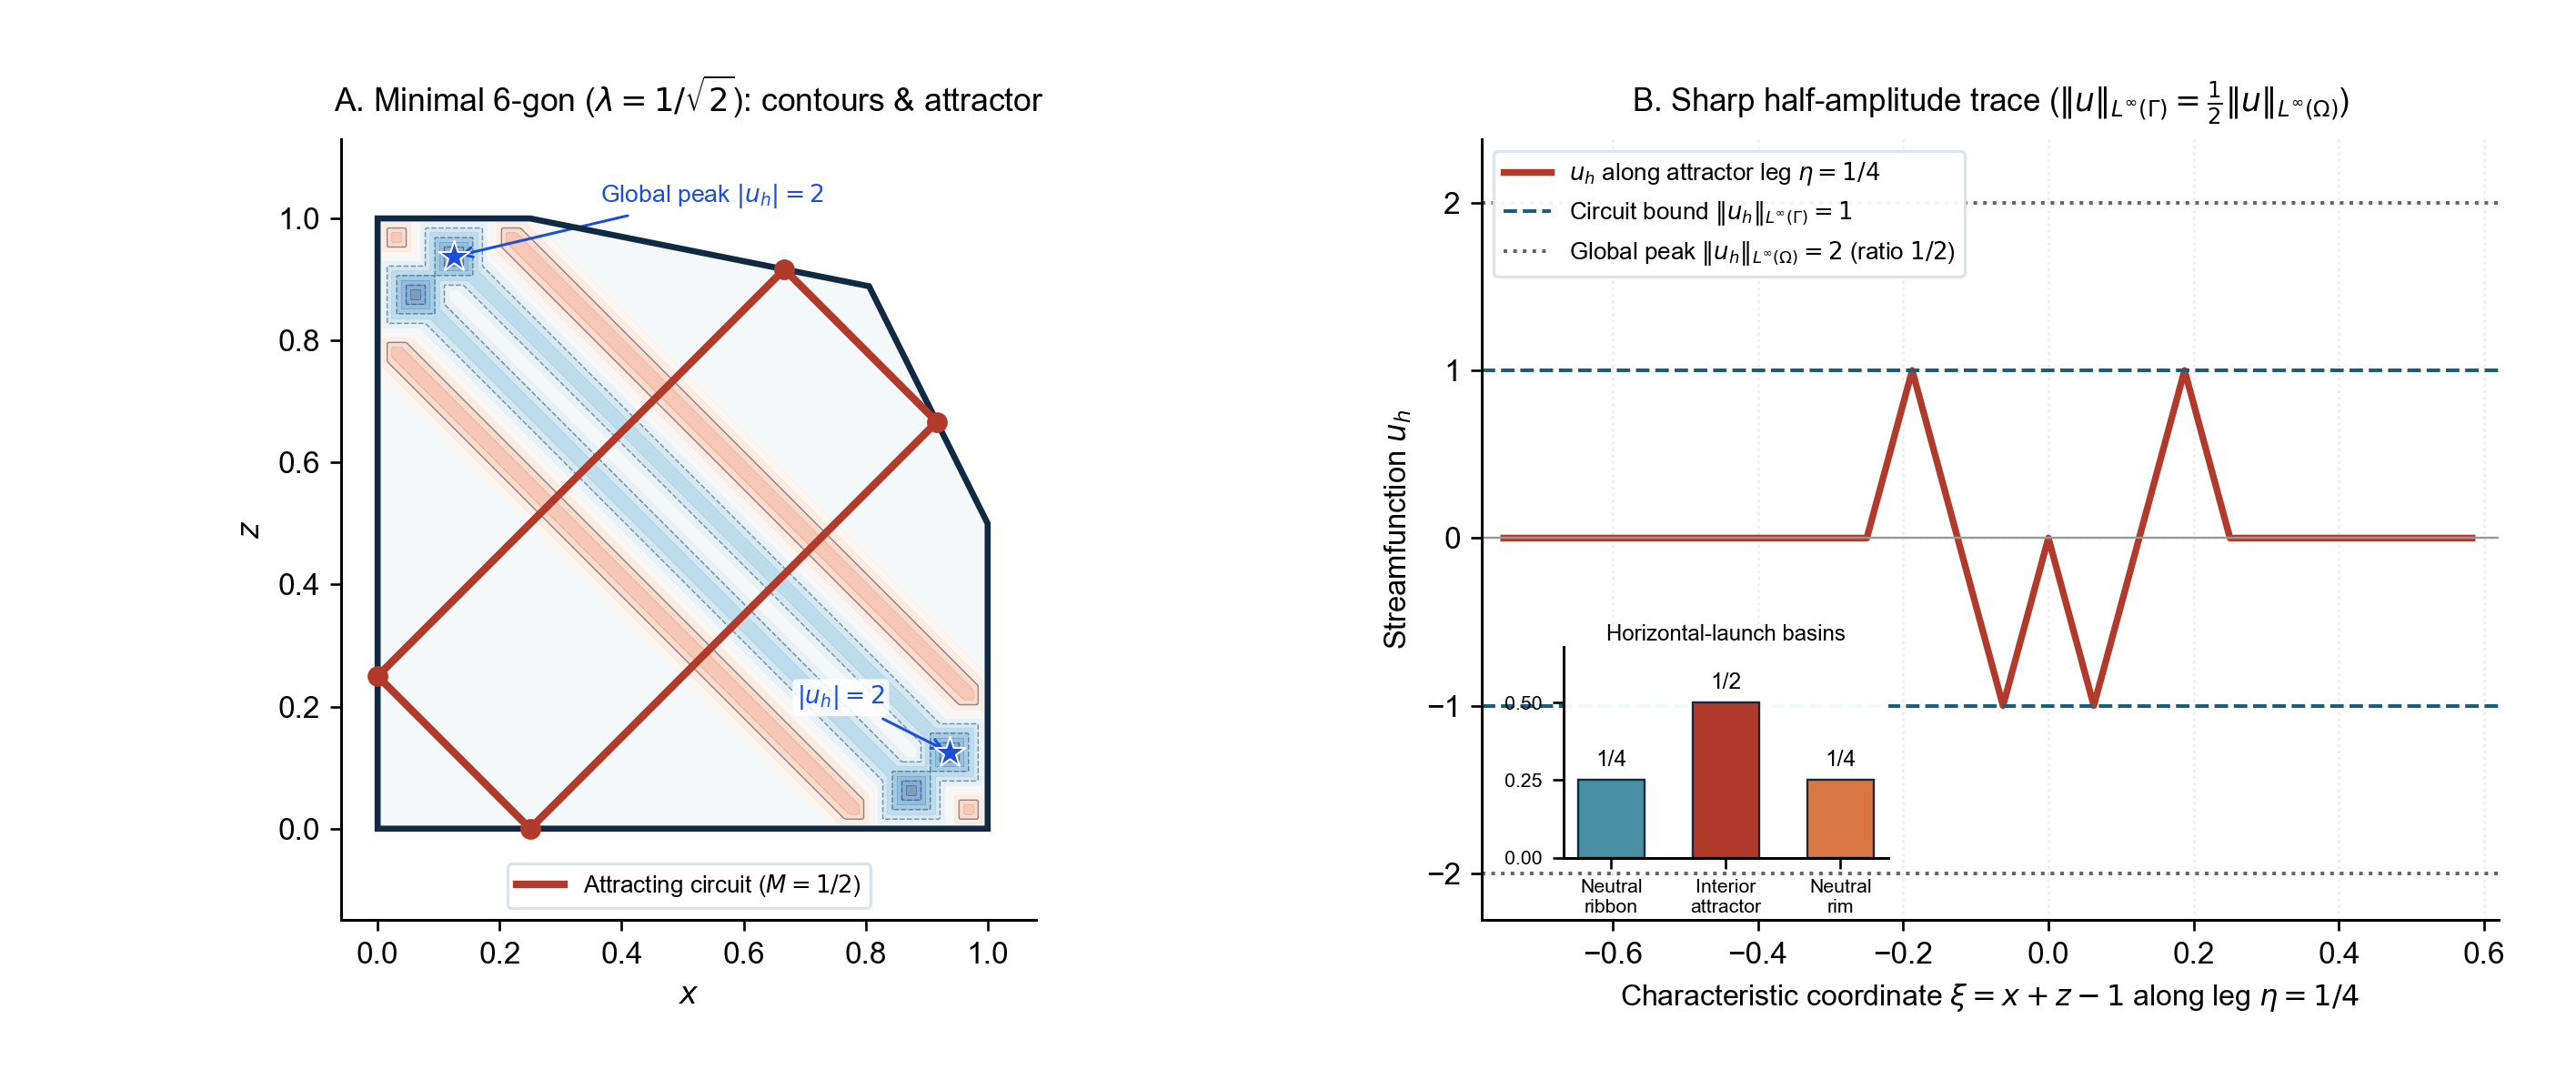
\includegraphics[width=\textwidth]{figs/p1_fig1_hexagon_uncloakability.png}
\caption{\textbf{A.} Minimal period-two coexistence hexagon with rational vertices at $\lambda = 1/\sqrt{2}$ showing streamfunction contours of the sharp piecewise-linear mode $u_h$ (global peaks $|u_h| = 2$ marked by stars) traversed by the attracting four-bounce circuit $\Gamma$ (multiplier $M = 1/2$). \textbf{B.} Trace of $u_h$ along the attractor leg $\eta = 1/4$, saturating the universal bound $\|u_h\|_{L^\infty(\Gamma)} = 1 = \frac{1}{2}\|u_h\|_{L^\infty(\Omega)}$; inset shows the exact horizontal-launch basin fractions $(1/4, 1/2, 1/4)$.}
\label{fig:p1-fig1}
\end{figure}

% ==============================================================================
\section{Finite-Energy Eigenmodes, Common-Extremum Annihilation, and Orthogonal Polyominoes}\label{sec:pde}
% ==============================================================================

We begin by making Aleksandryan's boundary reduction completely rigorous in the energy space $H_0^1(\Omega)$ on polygons, where corners and characteristic-parallel faces violate the $C^\infty$ strict-convexity hypotheses of \cite[\S 4, p.~482]{Aleksandryan1960}.

\subsection{The exact \texorpdfstring{$H_0^1$}{H01} boundary-profile criterion}
For $0 < \lambda < 1$, let $s = \sqrt{1-\lambda^2}/\lambda > 0$, $\xi = z + sx$, and $\eta = z - sx$. Note first that the spectral endpoints $E = 0$ and $E = 1$ are never eigenvalues of $T = \Delta_D^{-1}\partial_z^2$ on any bounded domain $\Omega$: indeed $\langle Tu, u \rangle_{H_0^1} = \|u_z\|_{L^2(\Omega)}^2$ and $\langle (I-T)u, u \rangle_{H_0^1} = \|u_x\|_{L^2(\Omega)}^2$, so extending $u \in H_0^1(\Omega)$ by zero outside $\Omega$ and slicing along horizontal or vertical lines forces $u = 0$ if either derivative vanishes identically.

On a convex polygon $K = \overline{\Omega}$ (adjacent collinear edges merged), define the boundary involutions $r_\xi, r_\eta \colon \partial K \to \partial K$ preserving $\xi$ and $\eta$ respectively (so $r_\xi = \gamma_\lambda^+$ and $r_\eta = \gamma_\lambda^-$). At a unique extremal vertex of $\xi$ (or $\eta$), the corresponding involution fixes that vertex. Along a whole characteristic supporting side (where $\xi$ or $\eta$ is constant), define the involution by reflection in the side's midpoint; this makes $r_\xi$ and $r_\eta$ orientation-reversing piecewise-affine homeomorphisms of $\partial K$, and $b = r_\xi r_\eta$ an orientation-preserving circle homeomorphism.

\begin{theorem}[Complete $H_0^1$ polygonal eigenmode criterion]\label{thm:h1-criterion}
For every bounded convex polygon $K = \overline{\Omega}$ and every $\lambda \in (0,1)$, the complex eigenspace $\ker(T - \lambda^2) \subset H_0^1(\Omega)$ is naturally isomorphic to the quotient profile space
\begin{equation}\label{eq:h1-space}
  \mathcal{H}_\lambda(\partial K) = \Bigl\{ H \in H^1(\partial K; \C) : H \circ r_\xi = H \circ r_\eta = H,\;\; H \text{ is constant on each characteristic side} \Bigr\} \Big/ \C
\end{equation}
(with $\C$ replaced by $\R$ for real-valued eigenmodes). Specifically, each representative $H$ of a class in $\mathcal{H}_\lambda(\partial K)$ factors uniquely as $H = A \circ \xi = B \circ \eta$ on $\partial K$ with $A, B$ in ordinary $H^1$ on their full bounded projection intervals $\xi(K), \eta(K)$ (so the class determines $(A, B)$ up to a common additive constant), and the corresponding streamfunction $u(x,z) = A(\xi) - B(\eta)$ depends only on the class of $H$ and belongs to $H_0^1(\Omega) \cap C(\overline{\Omega})$ with zero Dirichlet trace.
\end{theorem}

\begin{proof}
Suppose $u \in H_0^1(\Omega)$ satisfies $(1-\lambda^2)u_{zz} - \lambda^2 u_{xx} = 0$ distributionally. In characteristic coordinates $(\xi,\eta)$, $\partial_\eta u_\xi = 0$ in $\mathcal{D}'(\Omega)$, so on every open interior axis-aligned rectangle $u_\xi \in L^2$ depends only on $\xi$. Covering $\Omega$ by countably many interior rectangles and using the connectedness of each vertical slice $\Omega \cap \{\xi = \text{const}\}$ glues these representatives into a single function $a(\xi)$ with $u_\xi = a(\xi)$ a.e. Similarly $u_\eta = -b(\eta)$ a.e. Taking one-variable primitives and using connectedness of $\Omega$ gives $u = A(\xi) - B(\eta)$ with $A, B \in H^1_{\mathrm{loc}}$ on the open projection intervals. Writing $w_\xi(t)$ and $w_\eta(t)$ for the lengths of the $\xi$- and $\eta$-cross sections in $(\xi,\eta)$-coordinates, the invertible linear change of variables implies
\begin{equation}\label{eq:weighted-energy}
  \int_{\xi(\Omega)} w_\xi(t) |A'(t)|^2 \, dt + \int_{\eta(\Omega)} w_\eta(t) |B'(t)|^2 \, dt \le C_\lambda \|\nabla u\|_{L^2(\Omega)}^2 < \infty.
\end{equation}
Since $u \in H_0^1(\Omega)$, its zero trace on the relative interior of any transverse side forces $A(\xi) = B(\eta)$ pointwise along that open side (away from projection extrema) by continuity of local $H^1$ representatives.

It remains to verify ordinary $H^1$ regularity up to every endpoint of $\xi(K)$ and $\eta(K)$. By symmetry of $\xi$ and $\eta$, three mutually exhaustive configurations occur at an endpoint $\xi_{\mathrm{end}}$ of $\xi(K)$:
\begin{enumerate}
  \item \emph{Characteristic supporting side}: If $\xi = \xi_{\mathrm{end}}$ on a boundary edge $e$ of positive length, then $w_\xi(t)$ is bounded away from zero near $\xi_{\mathrm{end}}$, so \eqref{eq:weighted-energy} puts $A$ in ordinary $H^1$ up to $\xi_{\mathrm{end}}$. Continuity and the zero trace along $e$ force $B(\eta) = A(\xi_{\mathrm{end}})$ identically on $e$.
  \item \emph{Single extremal vertex $v$ with $B$ already $H^1$ near $\eta(v)$}: At least one incident side at $v$ is transverse to $\eta$, identifying $A$ with $B$ near $v$ via a nondegenerate affine reparametrization, so $A \in H^1$ up to $\xi(v)$. This covers every case where $\eta(v)$ is interior to $\eta(K)$ or lies on a characteristic $\eta$-side (by Case~1).
  \item \emph{Common extremal vertex}: Suppose $v$ uniquely realizes extrema of both $\xi$ and $\eta$. Translate $v$ to $(0,0)$ and flip coordinate signs if needed so $K$ lies in the first quadrant bounded near the origin by two incident edges $\eta = a\xi$ and $\eta = d\xi$ with $0 < a < d$. The zero trace on both edges yields $B(a\xi) = A(\xi) = B(d\xi)$ for all small $\xi > 0$. Setting $k = a/d \in (0,1)$, we have $B(ky) = B(y)$ for $y \in (0,c]$, while the slice width is $w_\eta(y) = (a^{-1} - d^{-1})y$. Changing variables $y \mapsto ky$ shows that every geometric shell $[k^{j+1}c, k^j c]$ contributes the identical integral
  \[
    \int_{k^{j+1}c}^{k^j c} y |B'(y)|^2 \, dy = \int_{kc}^{c} y |B'(y)|^2 \, dy \qquad (j \ge 0).
  \]
  (Notice that the linear weight $y$ alone permits divergent functions such as $\log\log(1/y)$; the boundary scaling identity $B(ky) = B(y)$ is indispensable.) Finiteness of the sum \eqref{eq:weighted-energy} forces each shell integral to vanish, so $B$---and hence $A$---is constant near the corner.
\end{enumerate}
Hence both $A$ and $B$ belong to ordinary $H^1$ on their full closed projection intervals and extend continuously to the endpoints, defining a single continuous $H \in H^1(\partial K)$ invariant under $r_\xi, r_\eta$ and constant on every characteristic side. Conversely, any $H \in \mathcal{H}_\lambda(\partial K)$ is constant on every fiber of $\xi|_{\partial K}$ and $\eta|_{\partial K}$, so composing with the piecewise-affine inverses along the monotone boundary chains produces $A, B \in H^1$ whose difference $u = A(\xi) - B(\eta)$ belongs to $H_0^1(\Omega) \cap C(\overline{\Omega})$, solves $u_{\xi\eta} = 0$, and vanishes iff $H$ is constant.
\end{proof}

\begin{theorem}[Periodic-interval spectral characterization]\label{thm:periodic-interval}
Let $E \subset \partial K$ denote the union of all closed characteristic sides of $K$ at slope $s = \sqrt{1-\lambda^2}/\lambda$. Then $\ker(T - \lambda^2) \ne \{0\}$ if and only if there exist an integer $q \ge 1$ and a nonempty open boundary arc $\mathcal{C} \subset \partial K$ such that $b^q|_{\mathcal{C}} = \Id$ and the full dihedral orbit $\bigcup_{j=0}^{q-1} (b^j \mathcal{C} \cup r_\eta b^j \mathcal{C})$ is disjoint from $E$. Whenever such an arc $\mathcal{C}$ exists, $\ker(T - \lambda^2)$ contains an infinite-dimensional subspace of $C^\infty(\overline{\Omega})$ modes supported in the union of the characteristic strips swept out by the reflected orbit.
\end{theorem}

\begin{proof}
(\emph{Necessity}) Suppose $H \in \mathcal{H}_\lambda(\partial K)$ is nonconstant; replacing $H$ by $\operatorname{Re}(e^{i\alpha} H)$ if complex, assume $H$ is real-valued. Choose $\delta > 0$ and a connected component $I$ of a strict superlevel set $\{H > c\}$ on which $\operatorname{osc}_I H > \delta$. Every forward image $b^n(I)$ is also a component with oscillation $> \delta$; by uniform continuity of $H$ on $\partial K$, the lengths of $b^n(I)$ have a uniform positive lower bound, so two images coincide and the endpoints of $I$ are periodic under $b$.

Let $q \ge 1$ be the common least period of periodic points of the orientation-preserving piecewise-affine circle homeomorphism $b$. Since $b^q$ has finitely many affine pieces, $\Fix(b^q)$ is a finite union of isolated points and closed intervals. On every open complementary gap of $\Fix(b^q)$, iterates of $b^q$ move monotonically to an endpoint, so continuity and $b$-invariance force $H$ to be constant on each closed gap. Thus $H$ can vary only on the interior of closed periodic intervals of $\Fix(b^q)$. Because the dihedral group generated by $r_\xi, r_\eta$ reduces to at most $2q$ sheets on $\Fix(b^q)$, the union of translates of $E$ intersects the interior of $\Fix(b^q)$ in a finite union of closed intervals and points, on each of which $H$ is constant. Since $H$ is nonconstant, some open subarc $\mathcal{C} \subset \Fix(b^q)$ must lie strictly outside all dihedral translates of $E$.

(\emph{Sufficiency}) Given such an open arc $\mathcal{C}$, let $q_0 \mid q$ be the primitive period of periodic points of the orientation-preserving circle homeomorphism $b$ (the denominator of its rational rotation number), so that $b^{q_0}|_{\mathcal{C}} = \Id$ and the full dihedral orbit of $\mathcal{C}$ is still disjoint from $E$. Pick $p_0 \in \mathcal{C}$ whose $2q_0$-point dihedral orbit avoids all polygon vertices, all breakpoints of the $2q_0$ sheet maps, and the finitely many fixed points of the orientation-reversing involutions $r_\eta b^j$ ($0 \le j < q_0$). Then the $2q_0$ points $b^j(p_0), r_\eta b^j(p_0)$ ($0 \le j < q_0$) are pairwise distinct (if $b^i(p_0) = r_\eta b^j(p_0)$, then $r_\eta b^{j+i}(p_0) = p_0$, excluded). Choosing a sufficiently short open subinterval $J \subset \mathcal{C}$ around $p_0$ makes the $2q_0$ sheets $b^j(J), r_\eta b^j(J)$ pairwise disjoint and affine, bounded away from all projection extrema and characteristic edges. Transporting any $f \in C_c^\infty(J)$ identically across all $2q_0$ sheets and extending by zero produces a smooth representative $H$ of a class in $\mathcal{H}_\lambda(\partial K)$ whose profiles $A, B$ are $C^\infty$ and compactly supported inside the open projection intervals. Hence $u = A(\xi) - B(\eta) \in C^\infty(\overline{\Omega}) \cap \ker(T - \lambda^2)$, and $f \mapsto u$ is injective.
\end{proof}

\subsection{Common-extremum annihilation: triangles, diamonds, and critical traps}
Theorem~\ref{thm:periodic-interval} shows why global periodicity of the midpoint-extended boundary map $b$ at a characteristic edge does \emph{not} suffice for an eigenmode: characteristic sides force boundary constancy and can collapse the entire kernel. A clean geometric obstruction unifies all such cases.

\begin{theorem}[Common-extremum annihilation]\label{thm:common-extremum}
If the characteristic-coordinate polygon $K_{\xi,\eta}$ contains any corner of its axis-aligned bounding box $[\xi_{\min},\xi_{\max}] \times [\eta_{\min},\eta_{\max}]$ (allowing either supporting face to be a whole characteristic side), then $\ker(T - \lambda^2) = \{0\}$. Consequently:
\begin{enumerate}
  \item Every triangle $\Omega \subset \R^2$ satisfies $\sigma_p(T) = \varnothing$ (including edge-parallel angles).
  \item Every axis-diagonal diamond $\{|x|/a + |z|/b < 1\}$ ($a, b > 0$) satisfies $\sigma_p(T) = \varnothing$.
\end{enumerate}
\end{theorem}

\begin{proof}
Translate and reflect $(\xi,\eta)$ so that $(0,0) \in K_{\xi,\eta} \subset [0,X] \times [0,Y]$. Define the piecewise-affine continuous boundary functions
\[
  l(t) = \min\{y : (t,y) \in K_{\xi,\eta}\}, \quad M(t) = \max\{y : (t,y) \in K_{\xi,\eta}\}, \quad m(y) = \min\{t : (t,y) \in K_{\xi,\eta}\}.
\]
By convexity and $(0,0) \in K_{\xi,\eta}$, $l$ is convex and nonnegative with $l(0) = 0$, hence nondecreasing. For every $t \in (0, X)$, the vertical slice has positive length $M(t) > l(t)$, so for $t' < t$ close to $t$ we have $l(t') \le l(t) < M(t')$, placing $(t', l(t))$ in $K_{\xi,\eta}$ and proving $T_0(t) := m(l(t)) \le t' < t$ (Figure~\ref{fig:p1-fig3}B). For any eigenmode $u = A(\xi) - B(\eta)$ from Theorem~\ref{thm:h1-criterion}, the zero boundary trace gives $A(t) = B(l(t)) = A(T_0(t))$ for all $t \in (0, X)$. Since $0 \le T_0(t) < t$ on $(0, X)$ and $T_0$ is continuous on $[0, X)$ with unique fixed point $0$ in $[0, X)$, for every $t \in (0, X)$ the iterates $T_0^n(t)$ decrease to $0$; continuity of $A$ therefore gives $A(t) = A(0)$ on $[0, X)$, and continuity at $X$ extends this to the closed interval $[0, X]$. Hence $B \equiv A(0)$ as well, whence $u \equiv 0$.

For any triangle, each linear functional $\xi$ and $\eta$ attains its minimum and maximum on at least two of the three vertices; by the pigeonhole principle their extremal sets intersect at a common weak extremum at every slope $s > 0$. For the axis-diagonal diamond $\{|x|/a + |z|/b \le 1\}$, the top and bottom vertices $(0,\pm b)$ realize the extrema of both $\xi$ and $\eta$ for $s < b/a$, the left and right vertices $(\pm a, 0)$ do so for $s > b/a$, and at the critical slope $s = b/a$ the domain becomes an axis-aligned rectangle in $(\xi,\eta)$ where all four corners are shared extrema.
\end{proof}

\begin{remark}[Historical scope and critical-edge counterexamples]
The absence of $H_0^1$ eigenmodes on triangles is credited to S.~D.~Troitskaya in \cite[\S 1.3]{DWZ2025} (see \cite{Troitskaya1999} for wedge uniqueness and \cite{Troitskaya2017} for basins with a sloping wall); Theorem~\ref{thm:common-extremum} gives a uniform elementary proof covering all critical angles simultaneously. Two explicit examples show that midpoint-extended global periodicity does not produce modes: at $s = 1$, the characteristic-coordinate triangle with vertices $(-1,0), (1,0), (0,1)$ (half of an upright square) has midpoint-extended map $b^2 = \Id$ everywhere, while $(0,0), (1,0), (0,1)$ satisfies $b^3 = \Id$ everywhere; in both cases Theorem~\ref{thm:common-extremum} forces $\ker(T - 1/2) = \{0\}$.
\end{remark}

\subsection{Nonconvex orthogonal polygons and polyominoes}
To contrast convex instability with orthogonal specular unfolding, consider a bounded, connected \emph{orthogonal polygonal domain} $\Omega \subset \R^2$ (possibly nonconvex and with polygonal holes) with Lipschitz boundary whose walls are horizontal or vertical.

\begin{theorem}[Orthogonal polygons and rectangular polyominoes]\label{thm:polyomino}
Let $\Omega \subset \R^2$ be a bounded connected orthogonal polygonal domain with Lipschitz boundary.
\begin{enumerate}
  \item For arbitrary positive edge lengths, the eigenvalues of $T$ having infinite multiplicity are dense in $[0,1]$.
  \item If all vertical and horizontal edges of $\Omega$ lie on a rectangular grid $x \in x_0 + a\Z$, $z \in z_0 + b\Z$ ($a, b > 0$), then the complete point spectrum (each eigenvalue of infinite multiplicity) is
  \begin{equation}\label{eq:polyomino-spec}
    \sigma_p(T) = \sigma_p(P) = \left\{ \frac{(n/b)^2}{(m/a)^2 + (n/b)^2} : m, n \in \N_{\ge 1} \right\}.
  \end{equation}
  In particular, every connected $a\times b$ grid polyomino with Lipschitz boundary has the exact same point spectrum and infinite eigenmultiplicities as the $a\times b$ mesh rectangle (matching the unit-square point spectrum if and only if $a/b \in \Q$, as for every square-grid polyomino such as the L-triomino).
  \item On the L-triomino $\Omega_L = ((0,2)\times(0,1)) \cup ((0,1)\times(0,2)) \setminus \{(1,1)\}$ (open interior), the separated grid sine products $\sin(m\pi x)\sin(n\pi z)$ are \emph{incomplete} in $H_0^1(\Omega_L)$.
\end{enumerate}
\end{theorem}

\begin{proof}
Reflecting $\Omega$ across horizontal and vertical walls produces a compact translation surface $X$ glued from four copies of $\Omega$, with commuting sign-flip isometries $H, V$ and half-turn $R = HV$ ($DR = -I$ in flat coordinates). For any direction $(1,s)$ carrying a regular closed geodesic on $X$, there is an open cylinder of parallel closed geodesics avoiding all cone points (vertex lifts). Choose a smooth transverse bump $f$ supported on a thin subcylinder disjoint from its image under $R$ (always possible even on an $R$-invariant cylinder since $R$ reverses the transverse coordinate). Setting $F = (I + R^*)f$ and $U = (I - H^*)F$ yields a smooth function solving $D_+ D_- U = 0$ ($D_\pm = \partial_x \pm s\partial_z$) that is odd under both $H$ and $V$, hence restricts to a smooth Dirichlet eigenmode on $\Omega$. Injectivity holds because $U = 0$ makes $F$ constant along both independent directions, hence constant on $X$, forcing $F = 0$ and $f = 0$ by disjointness of supports. Varying $f$ gives infinite multiplicity, and Masur's theorem \cite[Thms.~1--2]{Masur1986} supplies regular periodic directions in every open angular interval, proving~(1).

For~(2), every value in \eqref{eq:polyomino-spec} is realized with infinite multiplicity by the grid modes $\sin(k m\pi(x-x_0)/a)\sin(k n\pi(z-z_0)/b)$ ($k \ge 1$), which are linearly independent on any open mesh cell. Conversely, let $u \in \ker(T - \lambda^2) \subset H_0^1(\Omega)$ and extend $u$ oddly across the horizontal and vertical walls to $U \in H^1(X)$. Testing against differences of smooth functions supported across any open wall shows that $D_+ D_- U = 0$ distributionally away from the finite set of cone points. In flow boxes, $D_- U \in L^2(X)$ is constant a.e.\ along $D_+$ trajectories, and $D_+ U$ along $D_-$ trajectories (singular trajectories through cone points have measure zero). Rescaling $(x,z)$ to the unit mesh makes $X$ a square-tiled surface with directional slopes $\pm s a/b$. If $sa/b \notin \Q$, both straight-line flows are uniquely ergodic for flat area by the arithmetic Veech dichotomy (cf.\ \cite[\S 1 and App.~C]{HubertLelievre2006}), forcing $D_- U$ and $D_+ U$ to be constant a.e. Since $U \circ R = U$ reverses the sign of $D_\pm U$, both constants vanish, so $U$ is constant and oddness gives $U = 0$. Thus $\lambda^2 \in \sigma_p(T)$ implies $sa/b = m/n \in \Q_{>0}$, giving \eqref{eq:polyomino-spec}.

For~(3), every separated mode $\sin(m\pi x)\sin(n\pi z)$ vanishes identically along the interior cut $\{x = 1,\, 0 < z < 1\}$ (Figure~\ref{fig:p1-fig3}B, inset). By continuity of the local $H^1$ trace operator onto that interior segment, every function in their closed $H_0^1(\Omega_L)$ span vanishes along $\{x = 1,\, 0 < z < 1\}$, whereas a smooth bump supported in a small ball centered at $(1, 1/2)$ has nonzero trace there. (Whether the \emph{full} eigenspaces span $H_0^1(\Omega_L)$ remains open.)
\end{proof}

% ==============================================================================
\section{The Universal Half-Amplitude Uncloakability Theorem}\label{sec:uncloakability}
% ==============================================================================

When a convex polygon supports both a smooth standing eigenmode and a focusing wave attractor at the same frequency, physical intuition might suggest that the standing mode could remain trapped in an isolated neutral chamber with zero amplitude along the attracting ray. The following theorem proves that this is universally impossible.

\begin{theorem}[Universal Half-Amplitude Uncloakability]\label{thm:uncloakable}
Let $\Omega \subset \R^2$ be a bounded convex polygon and $\lambda \in (0,1)$ a noncharacteristic frequency at which the boundary map $b_\lambda = \gamma_\lambda^+ \gamma_\lambda^-$ has rational rotation number. Let $\Gamma \subset \overline{\Omega}$ denote the full spatial polygonal path of any regular periodic cycle of $b_\lambda$ with primitive boundary period $q \ge 2$. Then for every finite-energy standing mode $u \in \ker(T - \lambda^2) \subset H_0^1(\Omega)$ (evaluated via its continuous representative from Theorem~\ref{thm:h1-criterion}, with boundary profile representative $H \colon \partial\Omega \to \C$ and constant value $c_\Gamma = H|_{\Gamma \cap \partial\Omega}$),
\begin{equation}\label{eq:uncloakable-exact}
  \|u\|_{L^\infty(\Omega)} = \diam H(\partial\Omega), \qquad
  \|u\|_{L^\infty(\Gamma)} = \max_{w \in H(\partial\Omega)} |w - c_\Gamma| \ge \frac{1}{2}\|u\|_{L^\infty(\Omega)}.
\end{equation}
Equality $\|u\|_{L^\infty(\Gamma)} = \frac{1}{2}\|u\|_{L^\infty(\Omega)}$ holds if and only if $H(\partial\Omega) \subseteq \overline{D}\bigl(c_\Gamma,\, \frac{1}{2}\diam H(\partial\Omega)\bigr)$ in $\C$; for real-valued modes this is equivalent to $c_\Gamma = \frac{1}{2}(\min H + \max H)$, the midrange of $H(\partial\Omega)$. In particular, no nonzero standing mode can vanish identically along any coexisting regular periodic ray: every coexisting regular periodic circuit $\Gamma$ contains a point where $|u|$ is at least half the bulk maximum $\|u\|_{L^\infty(\Omega)}$.
\end{theorem}

\begin{proof}
Let $u = A(\xi) - B(\eta) \in C(\overline{\Omega})$ with common continuous boundary profile $H = A \circ \xi = B \circ \eta \in C(\partial\Omega; \C)$ from Theorem~\ref{thm:h1-criterion}. Since $A(\xi(\Omega)) \subset H(\partial\Omega)$ and $B(\eta(\Omega)) \subset H(\partial\Omega)$, every point $(x,z) \in \overline{\Omega}$ obeys $|u(x,z)| = |A(\xi) - B(\eta)| \le \diam H(\partial\Omega)$. Along $\Gamma$, every chord preserves either $\xi$ or $\eta$ and therefore fixes either $A(\xi) = c_\Gamma$ or $B(\eta) = c_\Gamma$, while the opposite coordinate takes values in $H(\partial\Omega)$; thus $|u(x,z)| \le \max_{w \in H(\partial\Omega)} |w - c_\Gamma|$ for all $(x,z) \in \Gamma$.

To prove the reverse inequalities, observe first that every value $w \in H(\partial\Omega)$ is attained on a periodic orbit of $b_\lambda$. Indeed, let $p \in \partial\Omega$ satisfy $H(p) = w$. Since $b_\lambda$ has rational rotation number with least period $q \ge 2$ (fixed by $\Gamma$), every point $p \notin \Fix(b_\lambda^q)$ lies in an open complementary gap whose forward iterates $b_\lambda^{nq}(p)$ converge monotonically to an endpoint $p_* \in \Fix(b_\lambda^q)$; by $b_\lambda$-invariance and continuity of $H$, $H(p_*) = w$.

Next, let $O_1$ and $O_2$ be any two distinct period-$q$ boundary orbits of $b_\lambda$ carrying distinct profile values $w_1 = H(O_1) \ne w_2 = H(O_2)$. Because $b_\lambda$ is an orientation-preserving circle homeomorphism of rotation number $p/q$ with $\gcd(p,q)=1$, the $q$ open boundary arcs between consecutive points of $O_1$ are permuted transitively by $b_\lambda$, so each arc contains exactly one point of $O_2$: the two orbits strictly interlace around $\partial\Omega$. Form the closed polygonal characteristic paths $\Gamma_1, \Gamma_2 \subset \overline{\Omega}$ by connecting the $2q$ successive chord endpoints of $O_1$ and $O_2$ (dropping any zero-length chord if an exceptional orbit passes through a supporting vertex). Since $O_1$ is connected by $\Gamma_1$, $O_2$ is connected by $\Gamma_2$, and $q \ge 2$, the interlacing of $O_1$ and $O_2$ furnishes an alternating quadruple $a_1, a_2, b_1, b_2$ in cyclic order on $\partial\Omega$ with $a_1, b_1 \in O_1$ and $a_2, b_2 \in O_2$.

We claim $\Gamma_1 \cap \Gamma_2 \ne \varnothing$. Suppose to the contrary that the compact connected sets $\Gamma_1$ and $\Gamma_2$ were disjoint. Since $\Omega$ is a convex topological disk and $\Gamma_1$ is a connected polygonal union of interior chords connecting $a_1$ to $b_1$ (meeting $\partial\Omega$ only at finitely many vertices/impacts), we could perturb a simple path inside $\Gamma_1$ from $a_1$ to $b_1$ slightly into $\Omega \setminus \Gamma_2$ while keeping its endpoints $a_1, b_1$ fixed; by the Jordan curve theorem this cross-cut separates $a_2$ from $b_2$ in $\overline{\Omega}$, contradicting the existence of a connected path $\Gamma_2$ from $a_2$ to $b_2$ disjoint from it.

Let $P = (x_*, z_*) \in \Gamma_1 \cap \Gamma_2$. The two paths cannot share a boundary impact point or a common characteristic segment (else $w_1 = H = w_2$ along that impact or line). Therefore $P$ is a transverse intersection of a chord of $\Gamma_1$ (say of constant $\xi$, so $A(\xi(P)) = w_1$) with a chord of $\Gamma_2$ (of constant $\eta$, so $B(\eta(P)) = w_2$), or vice versa. In either case $|u(P)| = |w_1 - w_2|$.

If $H$ is constant then $u \equiv 0$ and \eqref{eq:uncloakable-exact} holds trivially. Otherwise, by compactness of $H(\partial\Omega) \subset \C$, choose a diametral pair $w_-, w_+ \in H(\partial\Omega)$ attaining $|w_+ - w_-| = \diam H(\partial\Omega) > 0$; applying the intersection step to periodic orbits carrying $w_-$ and $w_+$ yields a point $P \in \Omega$ with $|u(P)| = |w_+ - w_-| = \diam H(\partial\Omega)$, establishing the first identity of \eqref{eq:uncloakable-exact}. Next, let $O_1 \subset \Gamma \cap \partial\Omega$ be one directed $b_\lambda$-orbit generating $\Gamma$ (so $\Gamma_1 = \Gamma$ and $H(O_1) = c_\Gamma$), and choose $w_2 \in H(\partial\Omega)$ maximizing $|w - c_\Gamma| > 0$. Applying the intersection step to $O_1$ and a periodic orbit carrying $w_2$ yields a point $P \in \Gamma$ with $|u(P)| = |w_2 - c_\Gamma| = \max_{w \in H(\partial\Omega)} |w - c_\Gamma|$, establishing the second identity. Finally, for any diametral pair $w_-, w_+ \in H(\partial\Omega)$ and any $c_\Gamma \in \C$,
\begin{align*}
  \max_{w \in H(\partial\Omega)} |w - c_\Gamma|
  &\ge \max(|w_+ - c_\Gamma|, |w_- - c_\Gamma|) \\
  &\ge \frac{|w_+ - c_\Gamma| + |c_\Gamma - w_-|}{2}
  \ge \frac{|w_+ - w_-|}{2} = \frac{1}{2}\diam H(\partial\Omega).
\end{align*}
Equality holds if and only if $|w - c_\Gamma| \le \frac{1}{2}\diam H(\partial\Omega)$ for every $w \in H(\partial\Omega)$, i.e., $H(\partial\Omega) \subseteq \overline{D}(c_\Gamma, \frac{1}{2}\diam H(\partial\Omega))$ (note that over $\C$, merely being the midpoint of one diametral pair is insufficient). For real-valued $H$, $H(\partial\Omega) = [\min H, \max H]$ is a closed real interval, so this disk containment reduces to $c_\Gamma = \frac{1}{2}(\min H + \max H)$.
\end{proof}

\begin{remark}[Sharpness and exact single-leg energy recovery]
On the minimal period-two coexistence hexagon with rational vertices of Section~\ref{sec:design} (Figure~\ref{fig:p1-fig1}), the continuous piecewise-linear profile $h \in H^1(3/4, 1)$ attaining values $(0, 1, 0, -1, 0)$ at $(3/4, 13/16, 7/8, 15/16, 1)$ gives an eigenmode $u_h(\xi,\eta) = h(1-|\xi|) - h(|\eta|) \in H_0^1(\Omega)$ with Dirichlet energy $4\int_{3/4}^1 |h'|^2\,dy = 256$, global peak $|u_h(1/16, 13/16)| = 2$, and circuit maximum $\|u_h\|_{L^\infty(\Gamma)} = 1 = \frac{1}{2}\|u_h\|_{L^\infty(\Omega)}$ (verified in Lean~4 by \texttt{sharpGlobalAmplitude} and \texttt{sharpCircuitAmplitude} in \texttt{Uncloakability.lean}). Smooth bump profiles attaining $\pm 1$ yield $C^\infty(\overline{\Omega})$ sharp witnesses. Moreover, on either horizontal attractor leg $J = [r-1,\, 1-a+n(a-r)] \times \{\pm r\}$ of the coexistence hexagons $\Omega_\kappa$ in Section~\ref{sec:design} (specifically $[-3/4,\, 7/12] \times \{\pm 1/4\}$ on the canonical example), $h(|\eta|) = 0$ and the $\xi$-interval strictly covers $[-(1-a), 1-a]$, so measuring $u_h$ along a \emph{single} physical attractor leg recovers the entire bulk Dirichlet energy exactly:
\[
  \int_\Omega |\nabla_{x,z} u_h|^2 \, dx\,dz = \sqrt{2} \int_J |\partial_{\mathrm{arc}} u_h|^2 \, d\mathrm{arc}, \qquad d\mathrm{arc} = \frac{|d\xi|}{\sqrt{2}}.
\]
\end{remark}

% ==============================================================================
\section{Sharp Multiplicity Bounds and Coexistence Obstructions}\label{sec:multiplicity}
% ==============================================================================

How many attracting wave-attractor circuits can coexist simultaneously inside a convex $k$-gon at a single frequency, and what is the geometric cost of also supporting a standing-wave beam? Nogueira and Troubetzkoy \cite[Prop.~11]{NogueiraTroubetzkoy2020} proved an upper bound of $3k-4$ on periodic cylinders (combining neutral and hyperbolic orbits). Isolating two-sided attracting cycles via dihedral gap pairing sharpens this bound drastically, yielding sharp, attained ceilings in the general and period-two coexistence regimes together with a universal mixed-dynamics upper bound across all periods.

\begin{theorem}[Universal $k-3$ bound across all periods]\label{thm:k-minus-3}
Let $K$ be a convex $k$-gon ($k \ge 3$) and $\lambda \in (0,1)$ a noncharacteristic frequency. Then the number $m$ of two-sided attracting periodic cycles of $b_\lambda = \gamma_\lambda^+\gamma_\lambda^-$ (of arbitrary period) satisfies
\begin{equation}\label{eq:k-minus-3}
  m \le k - 3.
\end{equation}
At a characteristic (edge-parallel) frequency, the same bound $m \le k-3$ holds for regular hyperbolic \emph{attracting} cycles avoiding every tangent chord (and separately for repelling cycles). For every $k \ge 4$, the bound \eqref{eq:k-minus-3} is attained at period two by a convex $k$-gon with rational vertices and $k-3$ distinct contraction factors $M_j = (2j-1)/(2j+1)$ ($1 \le j \le k-3$).
\end{theorem}

\begin{proof}
Suppose $K$ has no characteristic edge and $b = \gamma^+\gamma^-$ possesses $m \ge 1$ two-sided attracting cycles. Because both involutions reverse time ($\gamma^- b \gamma^- = \gamma^+ b \gamma^+ = b^{-1}$), $\gamma^-$ maps the $m$ attracting cycles to $m$ distinct repelling cycles. All $2m$ cycles share a common least period $q$ by the rotation-number theorem. If $b$ had a fixed point $x$, then $\gamma^- x = \gamma^+ x = x$ (as two non-parallel characteristic lines meet only at $x$), making every periodic orbit a fixed point equal to its own time reverse, which cannot be a two-sided attractor. Hence $q \ge 2$, and the four extremal vertices of $\xi$ and $\eta$ are pairwise distinct and disjoint from all $2mq$ marked points.

Label the $2mq$ marked points cyclically modulo $2mq$. Since $b$ acts as a cyclic shift $d$ of order $q$, we have $\gcd(d, 2mq) = 2m$, partitioning both the marked points and the open boundary gaps between consecutive marked points into $2m$ $b$-orbit classes indexed by $\Z/2m\Z$. Because $\gamma^-$ reverses cyclic order and exchanges every attracting orbit with a distinct repelling orbit, it acts on marked-orbit classes by $i \mapsto h - i \pmod{2m}$ with no fixed class, forcing $h$ to be odd. On the gap class immediately following mark $i$, $\gamma^-$ induces $i \mapsto h - i - 1 \pmod{2m}$, which fixes \emph{exactly two} gap classes, $(h-1)/2$ and $(h-1)/2 + m$, and pairs the remaining $2m - 2$ gap classes into $m-1$ disjoint swapped pairs. Since $\gamma^+ = b\gamma^-$, both involutions induce the identical pairing on gap classes.

Each of the four extremal vertices is fixed by $\gamma^+$ or $\gamma^-$ and therefore lies in one of the two fixed gap classes. We claim that every one of the $m-1$ swapped gap-class pairs must contain at least one additional polygon vertex. Otherwise, pick a gap $J$ in a vertex-free pair; then every image $b^i(J)$ and $\gamma^- b^i(J)$ lies in a single open edge, so every half-step of $b^q$ is affine across $J$. Because $b^q$ fixes both endpoints of $J$, an affine map fixing both endpoints is the identity on $J$, contradicting the attraction or repulsion at its endpoints. Counting the four disjoint extrema plus at least one vertex in each of the $m-1$ swapped pairs yields $k \ge 4 + (m-1) = m+3$.

At a characteristic frequency, any finite family of regular hyperbolic attracting cycles avoiding tangent chords retains its exact edge itineraries and strict attraction under an arbitrarily small perturbation of the slope $s$, reducing to the noncharacteristic bound; reversing time yields the separate bound for repellers.

To attain \eqref{eq:k-minus-3} for any $m = k-3 \ge 1$ at $s = 1$ ($\lambda = 1/\sqrt{2}$), set $C = 10(m+1)^2$, $a_j = (-1)^{j-1}(2j-1)$ ($1 \le j \le m$), and define in characteristic coordinates $(u,v) = (z+x, z-x)$ the convex region $L(v) \le u \le R(v)$ where
\begin{equation}\label{eq:sharp-k-minus-3-poly}
  L(v) = |v|, \qquad R(v) = C + \tfrac{1}{2}v - 2\sum_{a_j > 0} (v - a_j)_+ - 2\sum_{a_j < 0} (a_j - v)_+,
\end{equation}
with $r_+ = \max(r, 0)$. The left wall has one bend at $v = 0$, the concave right wall has $m$ bends at $a_j$ (slope dropping by $2$ at each), and for $|v| \le 2m$ we have $R(v) \ge C - m - 4m^2 > 2m$, so the outer tails meet $L$ at two distinct top and bottom vertices, giving $k = m + 3$ rational vertices and no characteristic edges. Inscribed characteristic rectangles correspond to zeros $t > 0$ of $D(t) = R(t) - R(-t)$. Since $D(0) = 0$ and $D'(t)$ alternates between $+1$ and $-1$ at $t = 1, 3, \dots, 2m-1$, there is an isolated regular rectangle at each $t = 2j$ ($1 \le j \le m$), with diagonal multiplier $M_{\mathrm{SW}} = -R'(-2j)/R'(2j) = (1 + 4\lfloor j/2 \rfloor)/(4\lceil j/2 \rceil - 1)$, giving attracting multipliers $M_j = \min(M_{\mathrm{SW}}, M_{\mathrm{SW}}^{-1}) = (2j-1)/(2j+1)$.
\end{proof}

\begin{remark}[Combined count at a characteristic edge]
At a characteristic frequency, the \emph{combined} count of regular attracting and repelling cycles can exceed $k-3$: truncating the $m=2$ pentagon \eqref{eq:sharp-k-minus-3-poly} by the characteristic wall $u \ge 1/2$ yields a convex hexagon ($k=6$) retaining both transverse rectangles $[2,89]\times[-2,2]$ and $[4,86]\times[-4,4]$, whose four directed cycles have multipliers $1/3, 3, 3/5, 5/3$ (two attractors and two repellers).
\end{remark}

\begin{theorem}[Mixed-dynamics bounds and period-two coexistence ceilings]\label{thm:mixed-bounds}
Let $K$ be a convex $k$-gon supporting both a nonzero standing-wave eigenspace $\ker(T-\lambda^2) \ne \{0\}$ (equivalently, an admissible neutral periodic cylinder) and $m \ge 1$ regular attracting cycles at the same frequency $\lambda \in (0,1)$.
\begin{enumerate}
  \item \textbf{Universal mixed upper bound (any period $q$)}: Necessarily $m \le k - 4$ (i.e., $k \ge m + 4$). In particular, \emph{no convex quadrilateral ($k = 4$) admits coexisting standing modes and regular attracting cycles at any frequency or period}. (Sharpness of $m \le k - 4$ for higher periods $q \ge 3$---in particular whether a convex pentagon admits mixed dynamics at some $q \ge 3$---remains open.)
  \item \textbf{Sharp period-two ceiling}: At a noncharacteristic frequency of period two, $m \le \max(0, k - 5)$; in particular $k \ge 6$ is minimal for period-two coexistence.
  \item \textbf{Sharp centrally symmetric period-two ceiling}: If $K$ is a centrally symmetric $2h$-gon at a noncharacteristic period-two frequency, then $m \le \max(0, h - 3)$; in particular $2h \ge 8$ is minimal.
\end{enumerate}
\end{theorem}

\begin{proof}
(\emph{Part 1}) Assume first that $\lambda$ is noncharacteristic. By Theorem~\ref{thm:periodic-interval}, $\ker(T-\lambda^2) \ne \{0\}$ supplies an open periodic interval $\mathcal{C} \subset \Fix(b^q)$. Choose $p \in \mathcal{C}$ whose full dihedral orbit avoids all vertices and the finitely many fixed points of the orientation-reversing involutions $\gamma^- b^j$ ($0 \le j < q$), and set $N = \operatorname{Orb}_b(p)$, so that $N$ and $\gamma^- N$ are distinct regular neutral orbits (whose points occupy the translates of $\mathcal{C}$). Adjoin $N$ and $\gamma^- N$ to the $m$ attracting and $m$ repelling orbits from the proof of Theorem~\ref{thm:k-minus-3}, giving $2(m+1)$ cyclic orbit classes. As before, $\gamma^-$ acts by $i \mapsto d - i$ with $d$ odd and fixes exactly two gap classes containing the four extremal vertices, while pairing the remaining $2m$ gap classes into $m$ swapped pairs. Could a non-fixed gap $J$ have both endpoints in the neutral classes $N, \gamma^- N$? No, because the two neutral classes are mutual $\gamma^-$-reverses, so any gap bordered by them has its gap class fixed by $\gamma^-$ and therefore belongs to one of the two fixed gap classes! Thus every one of the $m$ swapped gap pairs abuts at least one attracting or repelling mark; as in Theorem~\ref{thm:k-minus-3}, each swapped pair must therefore contain a vertex, giving $k \ge 4 + m$. If $\lambda$ is characteristic, a compact subbeam supporting smooth modes (disjoint from $E$ by Theorem~\ref{thm:periodic-interval}) and the $m$ regular attracting cycles have strictly positive clearance from all characteristic edges; perturbing only the characteristic wall lines slightly while fixing all other wall lines preserves all $m$ attractors and the neutral subbeam verbatim, reducing to the noncharacteristic bound. (For $k = 4$ at a characteristic angle, Theorem~\ref{thm:common-extremum} also directly forces $\ker(T-\lambda^2) = \{0\}$ since four supporting faces on four vertices with one face containing two vertices must share a weak extremum.)

(\emph{Part 2}) At a noncharacteristic period-two frequency, apply a linear map sending characteristic lines to coordinate axes. The signs of the outward edge normals partition the $k$ edges into four nonempty monotone chains (SW, SE, NE, NW) with edge counts $e_1 + e_2 + e_3 + e_4 = k$ and $\sum_{i=1}^4 (e_i - 1) = k - 4$ internal chain vertices. Writing $x(t), X(t)$ for the SW and SE abscissas at height $t$, and $w(x), v(X)$ for the NW and NE heights above $x, X$, a regular inscribed rectangle at bottom height $t$ satisfies $g(t) := v(X(t)) - w(x(t)) = 0$ with $x(t) < X(t)$ and $t < v(X(t))$. The continuous piecewise-affine function $g$ has breakpoints only where one of the four corners crosses an internal chain vertex, so $g$ has at most $P \le (k-4) + 1 = k - 3$ affine pieces. A neutral period-two cylinder forces $g \equiv 0$ on at least one whole piece, while every isolated regular attracting rectangle gives a strict interior zero of $g$ (endpoints have opposite strict signs). No affine piece adjacent to a zero piece can have endpoints of opposite strict signs; hence at least two pieces cannot carry strict interior crossings, leaving at most $\max(0, P - 2) \le \max(0, k - 5)$ attracting circuits.

(\emph{Part 3}) Put the center of $K$ at the origin and let $C = -I$. Since $b$ has rotation number $1/2$ and commutes with $C$ (a half-turn in normalized arclength), $Cb$ has rotation number $0$, so every period-two orbit satisfies $b(p) = -p$; hence every inscribed regular rectangle is centered at the origin, with corners $(\pm u, \pm v)$, $u, v > 0$. Represent $K$ as the intersection of its $h$ pairs of parallel supporting half-planes $|a_i u + \sigma_i b_i v| \le 1$, where $a_i, b_i > 0$ (by noncharacteristicity) and $\sigma_i \in \{+1, -1\}$. Along the rays $v = \pm t u$ ($t > 0$), the horizontal coordinates of $\partial K$ are $1/Q_\pm(t)$, where
\[
  Q_\pm(t) = \max_{1 \le i \le h} |a_i \pm \sigma_i b_i t|, \qquad E(t) := \max_{1 \le i \le h} (a_i + b_i t) = \max\{Q_+(t), Q_-(t)\}.
\]
Because $|a_i - b_i t| < a_i + b_i t$, we have $Q_+(t) = Q_-(t)$ iff both signs $\sigma_i = +1$ and $\sigma_i = -1$ attain the upper envelope $E(t)$ at $t$. An isolated regular rectangle corresponds to a breakpoint of $E(t)$ where two lines of opposite sign exchange dominance; a neutral cylinder yields an open interval on which $Q_+ \equiv Q_-$, requiring a single affine piece of $E(t)$ to be realized by \emph{two} strips of opposite signs. Because each strip supports at most one maximal piece of the convex envelope $E(t)$, this repeated piece leaves at most $P \le h - 1$ distinct affine pieces, and at least one of its at most $P - 1$ internal breakpoints abuts the neutral piece and cannot yield an isolated attractor. Thus $m \le \max(0, P - 2) \le \max(0, h - 3)$, forcing $h \ge 4$ ($2h \ge 8$) whenever $m \ge 1$.
\end{proof}

\begin{figure}[ht]
\centering
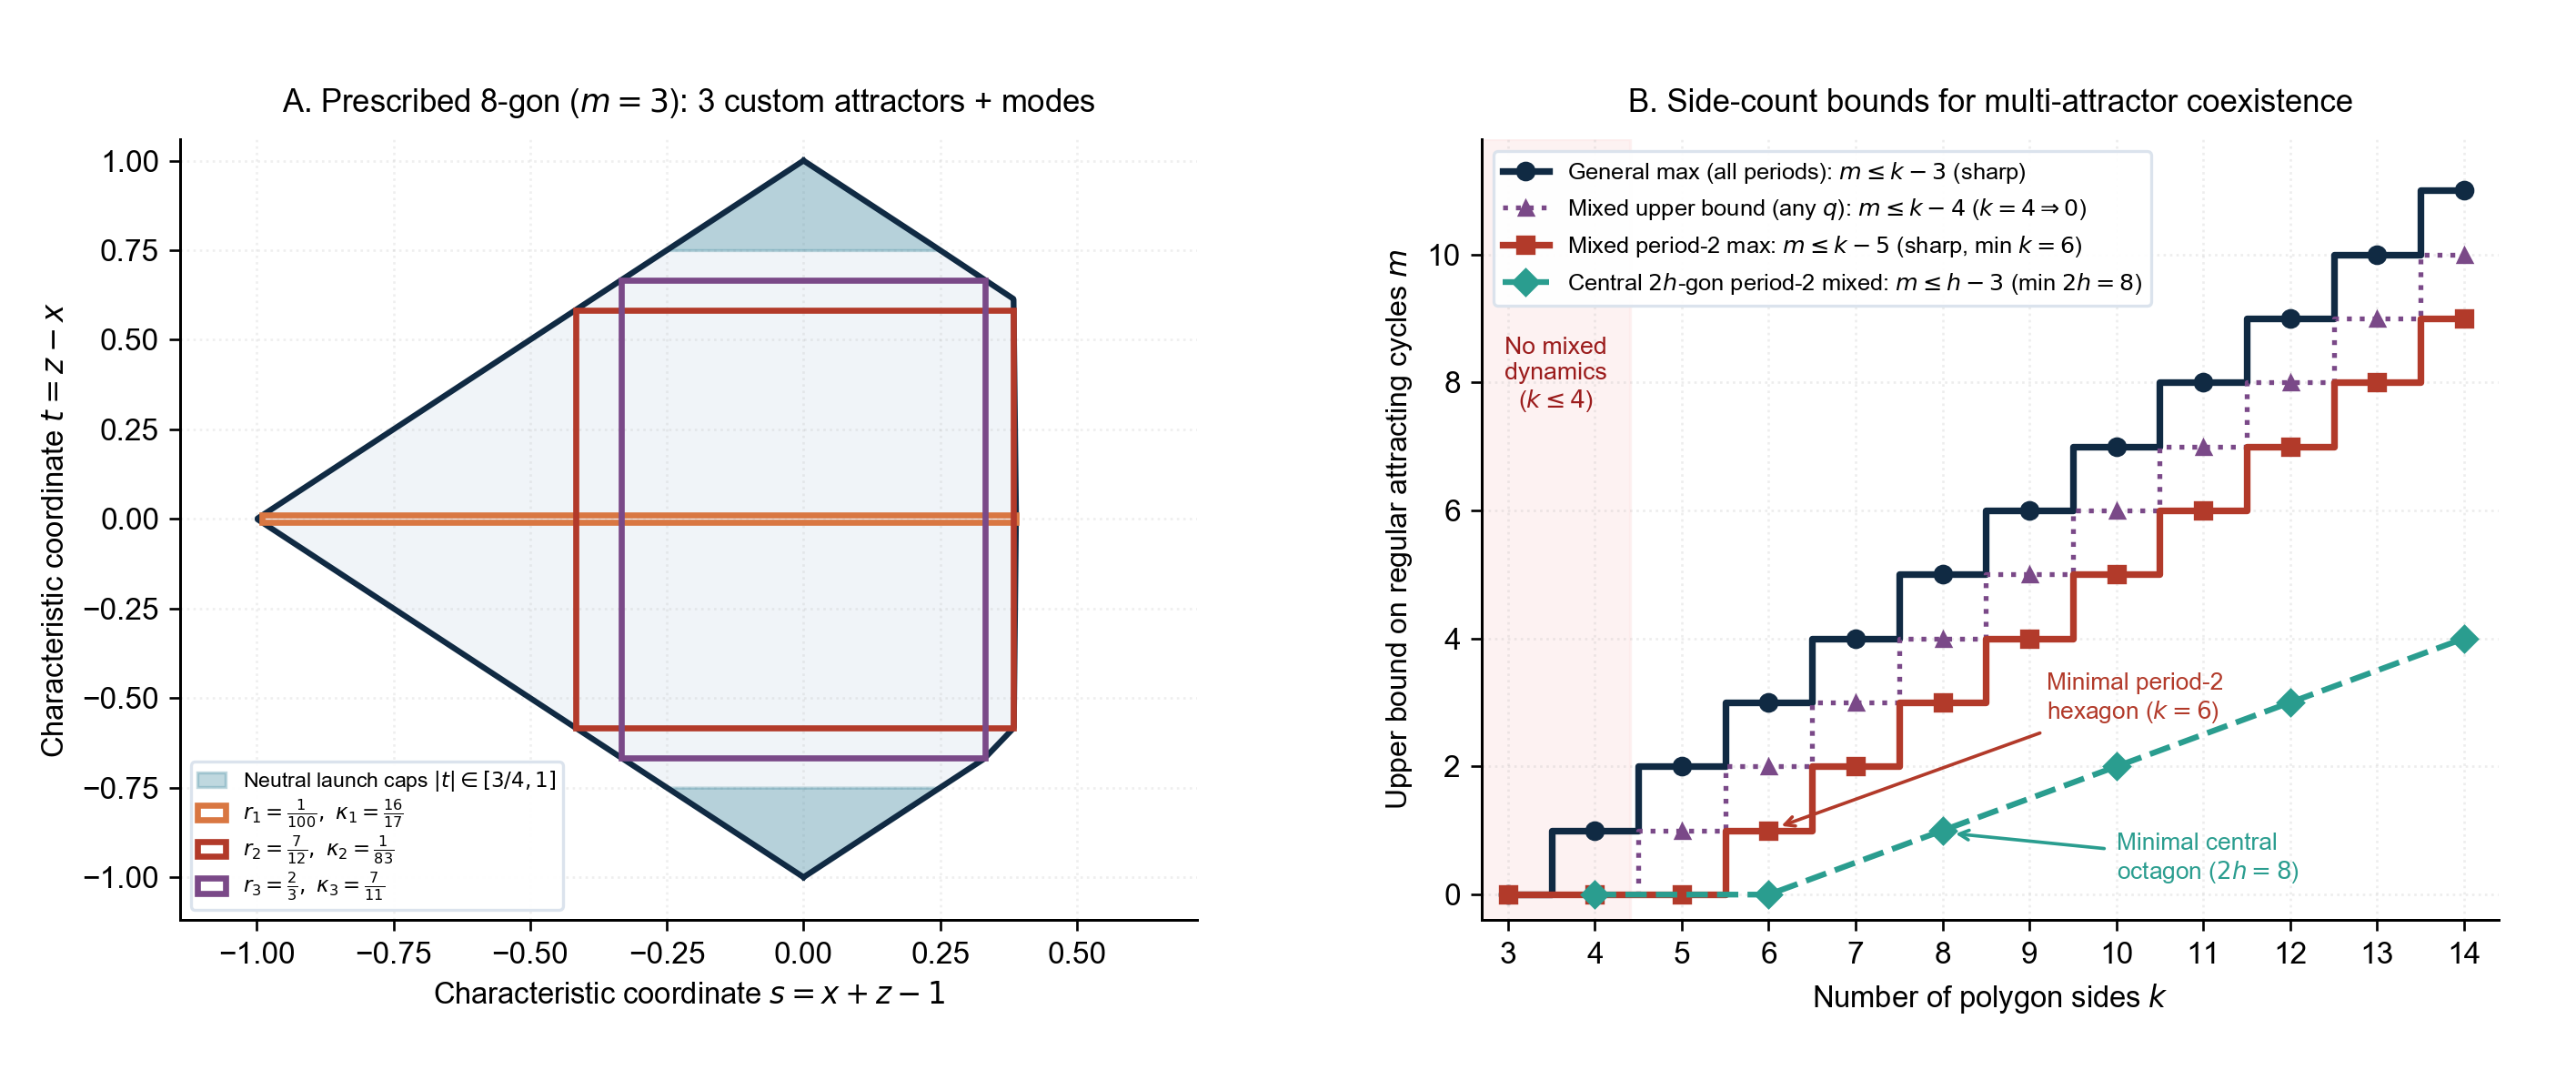
\includegraphics[width=\textwidth]{figs/p1_fig2_prescribed_multi_attractors.png}
\caption{\textbf{A.} Sharp prescribed-rate asymmetric convex octagon ($k = m + 5 = 8$, $m = 3$) in characteristic coordinates realizing three custom attracting circuits with independent heights $(1/100, 7/12, 2/3)$ and multipliers $(16/17, 1/83, 7/11)$ alongside the neutral horizontal-launch caps $|t| \in [3/4, 1]$ (whose vertical legs also sweep the central strip). \textbf{B.} Side-count bounds from Theorems~\ref{thm:k-minus-3} and~\ref{thm:mixed-bounds}: sharp general bound $m \le k-3$, arbitrary-period mixed upper bound $m \le k-4$ (excluding $k \le 4$; sharpness for $q \ge 3$ open), sharp period-two mixed ceiling $m \le k-5$ (minimal period-two hexagon), and sharp centrally symmetric period-two mixed ceiling $m \le h-3$ (minimal octagon).}
\label{fig:p1-fig2}
\end{figure}

\subsection{Regular-polygon saturation and symmetry-enforced rate pairing}
Remarkably, the universal bound $k-3$ of Theorem~\ref{thm:k-minus-3} is not merely achieved by custom polygons: it is already saturated by \emph{every} odd regular polygon with no characteristic edge at the half-frequency $\lambda = 1/\sqrt{2}$ ($s = 1$).

\begin{proposition}[Odd regular $N$-gons saturate $k-3$; symmetry pairing]\label{prop:odd-regular}
\leavevmode
\begin{enumerate}
  \item For every odd $N \ge 5$ and $s = 1$ ($\lambda = 1/\sqrt{2}$), a regular $N$-gon with no characteristic edge has \emph{exactly} $N - 3$ two-sided attracting period-two cycles and $\ker(T - 1/2) = \{0\}$. Reducing a characteristic-frame vertex angle to $\beta \in (0, \delta/2)$ with $\delta = \pi/N$, the $N - 3$ attracting multipliers are
  \begin{equation}\label{eq:odd-N-mult}
    M_\ell = \frac{\tan(t_\ell - a_\ell)\tan(t_\ell + b_\ell)}{\tan(t_\ell - b_\ell)\tan(t_\ell + a_\ell)}, \qquad t_\ell = \Bigl(1 + \frac{\ell}{2}\Bigr)\delta \qquad (0 \le \ell \le N-4),
  \end{equation}
  where $(a_\ell, b_\ell) = (\delta-\beta, \beta)$ for $\ell$ even and $(\delta/2+\beta, \delta/2-\beta)$ for $\ell$ odd. At the characteristic alignment $\beta = 0$, $\ker(T - 1/2)$ becomes infinite dimensional, while as $\beta \downarrow 0$ the $\ell = 0$ multiplier collapses as $M_0 \sim \beta\cot(2\delta) \to 0$ (exponent $\Lambda_0 \to -\infty$).
  \item Whenever a tank possesses a horizontal or vertical reflection symmetry $S$, the map $H = \gamma^+ S$ is an orientation-preserving circle homeomorphism satisfying $H^2 = b$. Consequently, every even-period regular attracting cycle is paired with a distinct attracting cycle having the \emph{exact same} Lyapunov exponent (for cycles passing through a breakpoint, the conjugation transports one-sided exponential rates identically). Regular hyperbolic exponents vary continuously under any perturbation preserving edge itineraries and can split once reflection symmetry is broken (as in the tilted pentagon of Figure~\ref{fig:p1-fig3}A).
\end{enumerate}
\end{proposition}

\begin{proof}
(\emph{Part 1}) Scale the apothem to $1$ in characteristic coordinates. Folding the $N$ unit outward normal angles $\beta + (2i+1)\delta$ into the first quadrant by taking component absolute values produces the strictly increasing cyclic-quadrant sequence $\beta$ (SW), $\delta-\beta$ (SE), $\delta+\beta$ (NE), $2\delta-\beta$ (NW), $2\delta+\beta$ (SW), \dots. Each of the $N - 3$ consecutive four-normal windows has folded arguments $t_\ell - a_\ell < t_\ell - b_\ell < t_\ell + b_\ell < t_\ell + a_\ell$ with $a_\ell + b_\ell = \delta$ and $\delta \le t_\ell \le \pi/2 - \delta$. Up to exchanging coordinate axes (which replaces $t_\ell$ by $\pi/2 - t_\ell$ and leaves $M_\ell$ invariant), the outer pair $t_\ell \pm a_\ell$ shares one folded first coordinate $x_{a_\ell}$ and the inner pair $t_\ell \pm b_\ell$ shares $x_{b_\ell}$, while the two lower normals share a folded ordinate $y - H$ and the two upper normals share $y + H$, where $H$ is their signed half-difference. Solving the four unit-tangent line equations uniquely yields $H = -K \sin a_\ell \sin b_\ell / \cos t_\ell < 0$ with $K = \sin(\delta/2) / [\cos\delta \cos((a_\ell-b_\ell)/2)]$, and every signed contact offset $w_\pm(r)$ ($r \in \{a_\ell, b_\ell\}$) from its edge midpoint obeys $\max(|w_+(r)|, |w_-(r)|) = \tan r + K\sin(\delta-r)(\tan r + \tan t_\ell) < \tan\delta$, because $\sin(\delta/2)\sin(t_\ell + r) < \cos(\delta/2)\sin\delta \le \cos((a_\ell-b_\ell)/2)\cos t_\ell$. Thus all four contacts lie strictly inside their assigned edges with strictly positive folded coordinates $x_r > 0$ and $y \pm H > 0$, unfolding to $N - 3$ distinct regular inscribed rectangles with attracting multipliers \eqref{eq:odd-N-mult} and saturating Theorem~\ref{thm:k-minus-3}. Furthermore, in any polygon circumscribed about the unit circle with distinct folded normal slopes, a continuum of inscribed rectangles would force two pairs of equal folded normals (since $G_h(t) = \sqrt{1+h^2 t^2} - h\sqrt{1+t^2}$ is strictly monotone for $h \ne 1$), excluding any neutral cylinder and forcing $\ker(T-1/2) = \{0\}$ (also implied directly by $m = N - 3 > N - 5$). At the critical alignment $\beta = 0$ (retaining apothem $1$, so the circumradius is $\sec\delta$), define the upper half-height $Y(u) = \max\{v : (u,v) \in K\}$; the vertical characteristic side has endpoint heights $\pm\tan\delta$, while a vertex within $\delta$ of the vertical axis has height at least $\sec\delta \cos\delta = 1 > \tan\delta$ (as $\delta \le \pi/5 < \pi/4$). Hence $w(u,v) = h(Y(u)) - h(|v|)$ for any $h \in C_c^\infty(\tan\delta, \max Y)$ supported away from vertex heights vanishes on the full boundary (including the vertical characteristic edge) and produces infinitely many independent $C^\infty$ eigenmodes.

(\emph{Part 2}) Because $S$ interchanges the $\xi$ and $\eta$ foliations, $S \gamma^- S = \gamma^+$, so $H^2 = \gamma^+ S \gamma^+ S = \gamma^+ \gamma^- = b$. Since $H$ commutes with $b$ and is piecewise-affine bi-Lipschitz (locally affine with nonzero derivative on regular orbits), $H$ preserves attraction and Lyapunov exponents (transporting one-sided rates at any breakpoint). If $H$ preserved a single even-period $q$-cycle, then $H = b^\ell$ on that cycle would require $2\ell \equiv 1 \pmod{q}$, impossible for even $q$.
\end{proof}

Table~\ref{tab:regular-multi} reports 85-digit outward-interval-verified exponents on regular $N$-gons (vertex angles $\alpha_j = \pi/2 + \phi + 2\pi j/N$), while Figure~\ref{fig:p1-fig3}A plots the binary64 continuation curve of the pentagon pair across $\phi \in [0^\circ, 5.5^\circ]$. On the regular pentagon ($s = 9/10$), the symmetric vertex-up orientation ($\phi = 0^\circ$) pairs both attractors at $\Lambda = -1.119139721$; tilting by $\phi = 5^\circ$ splits them with initial slope $d\Lambda/d\phi = \pm 8.161043\text{ rad}^{-1}$ into $-2.315915973$ and $-0.517344809$ (before characteristic alignment at $\phi = 5.9872^\circ$).

\begin{table}[ht]
\centering
\caption{85-digit outward-interval-verified period-two attracting exponents $\Lambda = \frac{1}{2}\log M$ on regular $N$-gons ($\alpha_j = \pi/2 + \phi + 2\pi j/N$). Counts saturate Theorem~\ref{thm:k-minus-3} for odd $N=5,9$ and the central bound $h-1$ for even $N=6,8,10$.}
\label{tab:regular-multi}
\footnotesize
\begin{tabular}{rrrrl}
\toprule
$N$ & $\phi$ & $s$ & Attractors & Certified per-step Lyapunov exponents $\Lambda$ \\
\midrule
$5$ & $0^\circ$ & $9/10$ & $2$ & $-1.119139721$ (paired twice by vertical symmetry) \\
$5$ & $5^\circ$ & $9/10$ & $2$ & $-2.315915973,\;\; -0.517344809$ (continuous split) \\
$6$ & $0^\circ$ & $9/10$ & $2$ & $-1.521438093$ (paired twice) \\
$6$ & $5^\circ$ & $9/10$ & $2$ & $-2.238415740,\;\; -0.989725581$ \\
$8$ & $5^\circ$ & $19/20$ & $3$ & $-1.307924075,\;\; -0.612922879,\;\; -0.394192178$ \\
$9$ & $0^\circ$ & $49/50$ & $6$ & $-0.853185884,\;\; -0.425836072,\;\; -0.390044045$ (each twice) \\
$10$ & $0^\circ$ & $19/20$ & $4$ & $-0.983975700,\;\; -0.712758345$ (each twice) \\
\bottomrule
\end{tabular}
\end{table}

\begin{figure}[ht]
\centering
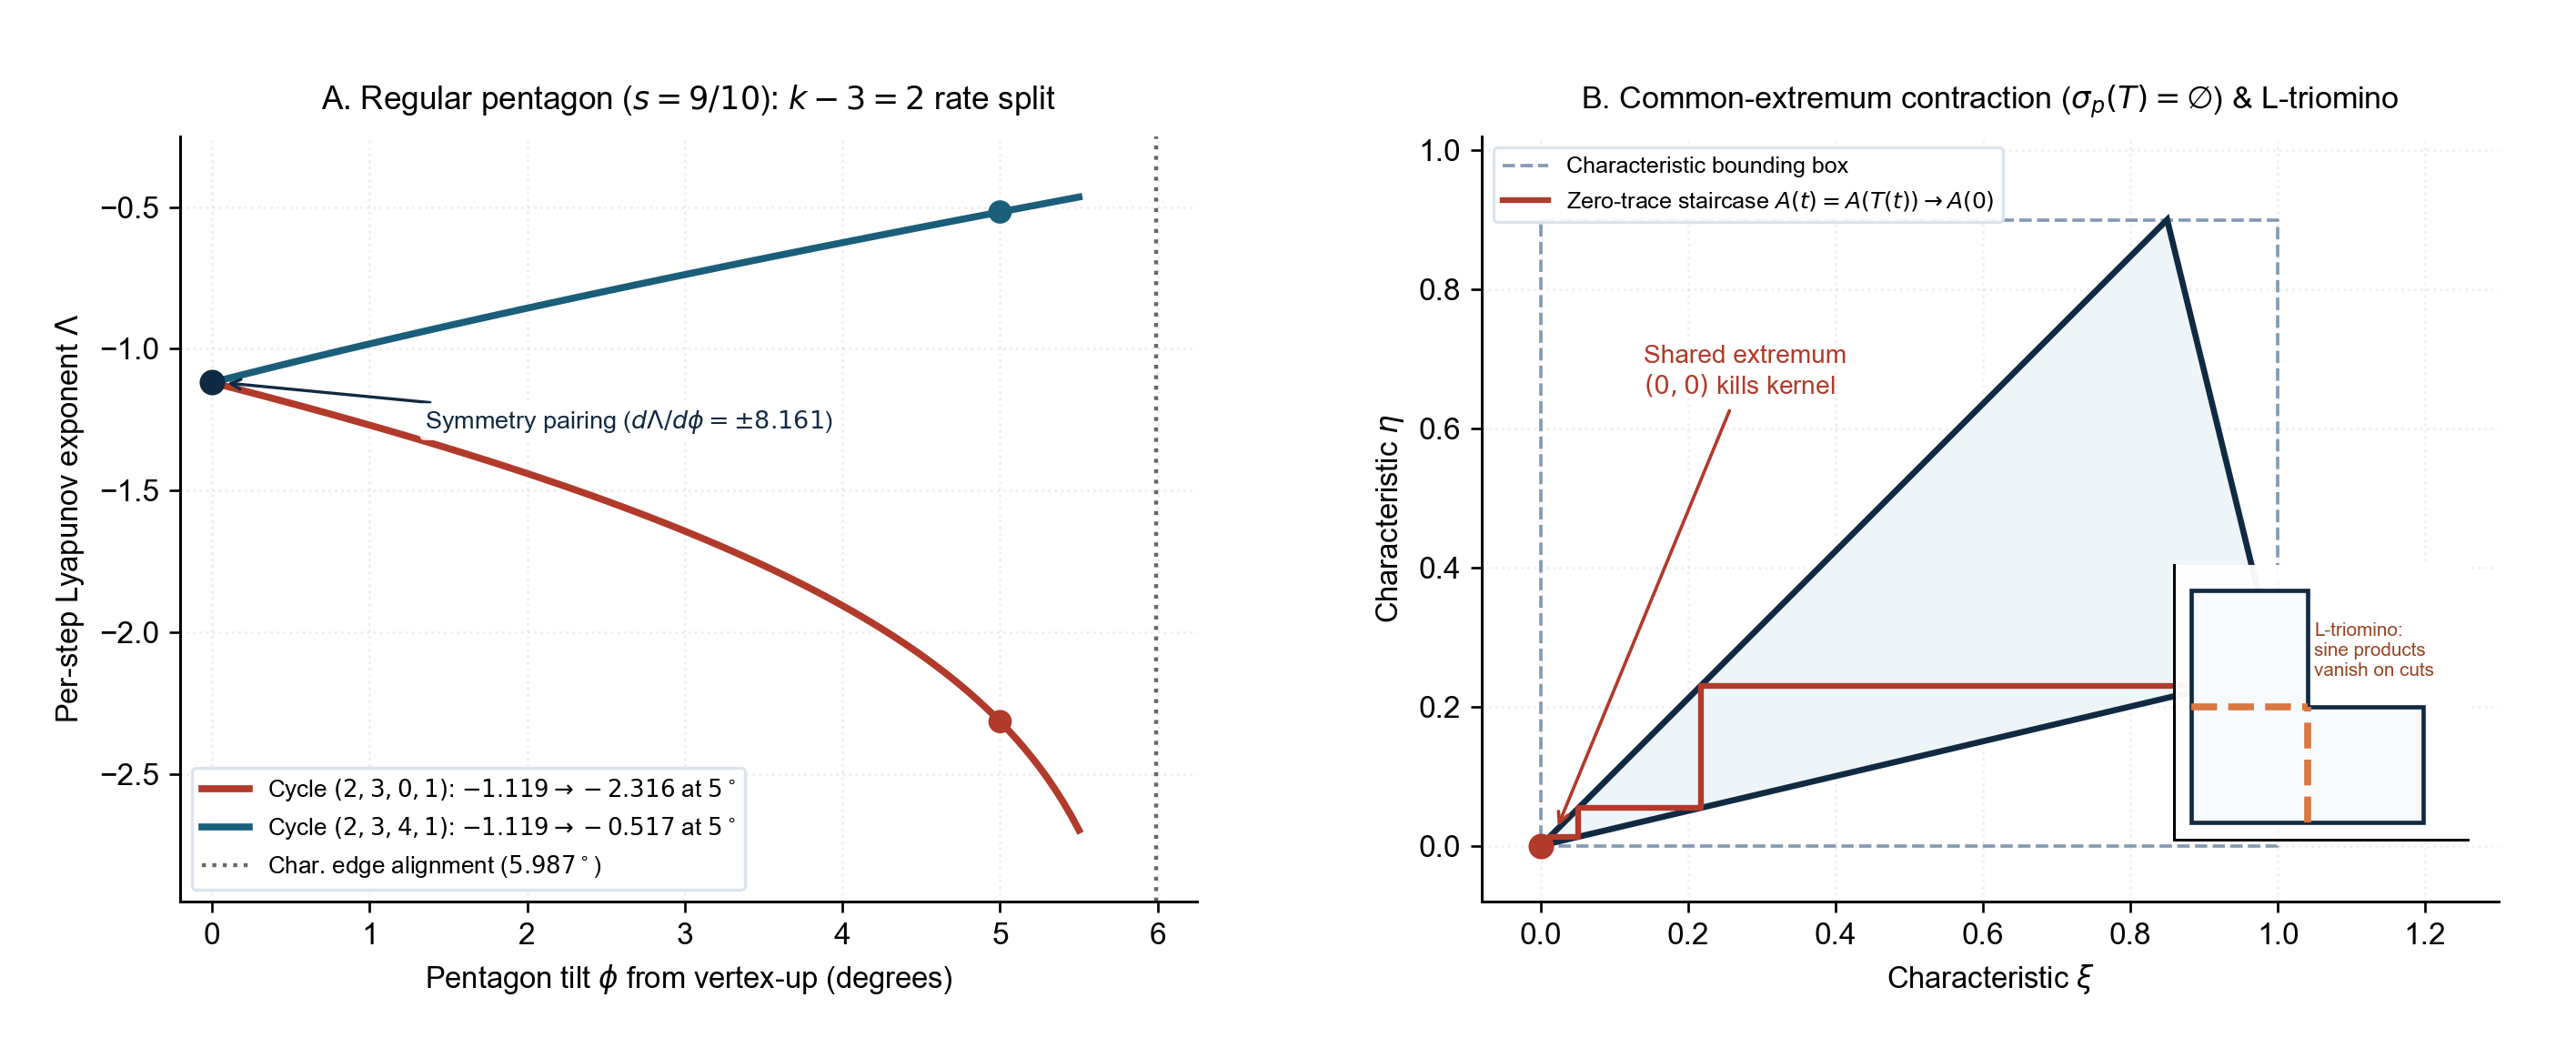
\includegraphics[width=\textwidth]{figs/p1_fig3_pentagon_and_obstructions.png}
\caption{\textbf{A.} Continuous rate splitting of the $k-3 = 2$ attracting cycles in the regular pentagon ($s = 9/10$) as tilt $\phi$ breaks vertical symmetry ($d\Lambda/d\phi = \pm 8.161\text{ rad}^{-1}$ at $\phi = 0^\circ$). \textbf{B.} Characteristic bounding-box staircase $A(t) = A(T_0(t)) \to A(0)$ proving Theorem~\ref{thm:common-extremum} ($\sigma_p(T)=\varnothing$ for all triangles); inset illustrates the interior trace cuts where separated sine products vanish on the L-triomino (Theorem~\ref{thm:polyomino}).}
\label{fig:p1-fig3}
\end{figure}

% ==============================================================================
\section{Prescribed-Rate Coexistence and Infinite-Rank Spectral Jumps}\label{sec:design}
% ==============================================================================

We now prove that the sharp side-count thresholds $k = m + 5$ and $2h = 2m + 6$ of Theorem~\ref{thm:mixed-bounds} are completely realizable with arbitrary prescribed locations and contraction factors, while keeping an entire infinite-dimensional eigenspace and its Dirichlet energy untouched.

\subsection{The minimal period-two hexagon, basins, and infinite-rank projection jump}
Set $s = 1$ ($\lambda = 1/\sqrt{2}$), characteristic coordinates $\xi = x + z - 1$, $\eta = z - x$ (equivalently physical coordinates $(x,z) \in [0,1]^2$ translated from the centered diamond). Fix a neutral cutoff $a \in (0,1)$, an attractor height $r \in (0,a)$, an outer slope $n \in (0,1)$, and a desired full-return contraction $\kappa \in (0,1]$. Define
\begin{equation}\label{eq:pivot-hex}
  m = \kappa n, \quad d = 1 - (1-n)a, \quad c = d - (n-m)r, \quad R_\kappa(\eta) = \min\{1 - |\eta|,\; c + m\eta,\; d - n\eta\},
\end{equation}
and consider the convex hexagon $\Omega_\kappa = \{|\eta| < 1,\; |\eta| - 1 < \xi < R_\kappa(\eta)\}$. Taking $(a, r, n, \kappa) = (3/4, 1/4, 2/3, 1/2)$ gives the canonical hexagon with rational vertices
\[
  R_{1/2}(\eta) = \min\!\left\{1 - |\eta|,\; \frac{2}{3} + \frac{\eta}{3},\; \frac{3}{4} - \frac{2\eta}{3}\right\},
\]
whose physical vertices in $[0,1]^2$ are $(0,0), (1,0), (1,1/2), (29/36, 8/9), (1/4,1), (0,1)$ (Figure~\ref{fig:p1-fig1}A). Geometrically, varying $\kappa \in (0,1]$ pivots a single straight cutting wall $\xi = c + m\eta$ around the fixed attractor impact point $(1 - a + n(a-r),\, -r)$ while holding the other five wall lines fixed.

\begin{theorem}[Minimal period-two hexagon coexistence, exact basins, and norm-one projection jump]\label{thm:hexagon-jump}
For every $\kappa \in (0,1)$, the convex hexagon $\Omega_\kappa$ at $\lambda = 1/\sqrt{2}$ satisfies:
\begin{enumerate}
  \item \textbf{Isolated attractor with prescribed rate}: The unique isolated nondegenerate four-bounce circuit is the fixed rectangle $[r-1,\, 1-a+n(a-r)] \times [-r, r]$ in $(\xi,\eta)$, with local left-wall return $y' = r + \kappa(y - r)$ and multiplier $\kappa$ (for the canonical hexagon with rational vertices, $y' = \frac{1}{8} + \frac{1}{2}y$, $\Lambda = -\frac{1}{2}\log 2$).
  \item \textbf{Complete eigenspace and fixed energy}: Extending $h \in H^1(a, 1)$ with $h(a) = 0$ by zero to $[0,a]$, the entire eigenspace $\ker(T_{\Omega_\kappa} - 1/2) \subset H_0^1(\Omega_\kappa)$ consists precisely of
  \begin{equation}\label{eq:exact-eigenspace}
    u_h(\xi,\eta) = h(1 - |\xi|) - h(|\eta|), \qquad \int_{\Omega_\kappa} |\nabla_{x,z} u_h|^2 \, dx\,dz = 4 \int_a^1 |h'(y)|^2 \, dy,
  \end{equation}
  independent of $\kappa \in (0,1)$ even after zero extension into a fixed ambient box $B \supset \bigcup_{\kappa \in (0,1]} \Omega_\kappa$.
  \item \textbf{Exact forward basins}: Under uniform horizontal launch offset $\eta \in [-1,1]$ with equally likely left or right wall, the basin weights are $1-a$ (neutral ribbon $|\eta| \in [a,1]$), $(a+r)/2$ (interior attracting circuit), and $(a-r)/2$ (convergence to the neutral-ribbon endpoint $\{P_R(-a), P_L(a)\}$), equaling $(1/4, 1/2, 1/4)$ on the canonical example.
  \item \textbf{Infinite-rank norm-one spectral jump}: As $\kappa \uparrow 1$, $\overline{\Omega_\kappa} \to \overline{\Omega_1}$ in Hausdorff distance, yet at $\kappa = 1$ the tank becomes symmetric ($b^2 = \Id$ globally) and its orthogonal complement $\ker(T_{\Omega_1} - 1/2) \ominus \ker(T_{\Omega_\kappa} - 1/2)$ is infinite dimensional, containing all smooth modes $g(1+\xi) + g((d-\xi)/n) - g(|\eta|)$ ($g \in C_c^\infty(0,a)$). Letting $\Pi_\kappa$ be the orthogonal projection in $H_0^1(B)$ onto the zero-extended eigenspace $\ker(T_{\Omega_\kappa} - 1/2)$,
  \begin{equation}\label{eq:proj-jump}
    \|\Pi_1 - \Pi_\kappa\| = 1, \qquad \rank(\Pi_1 - \Pi_\kappa) = \infty \qquad \forall \kappa \in (0,1).
  \end{equation}
\end{enumerate}
\end{theorem}

\begin{proof}
Direct subtraction of $R_\kappa(y) - R_\kappa(-y)$ for $y \in [0,1]$ yields the four-piece function
\[
  D_\kappa(y) =
  \begin{cases}
    2my, & 0 \le y \le \tau, \\
    (n-m)(r-y), & \tau \le y \le \beta, \\
    (1-n)(y-a), & \beta \le y \le a, \\
    0, & a \le y \le 1,
  \end{cases}
  \qquad \tau = \frac{n-m}{n+m}r < r < \beta = \frac{(1-n)a + (n-m)r}{1-m} < a.
\]
Hence the positive zeros of $D_\kappa$ are precisely $\{r\} \cup [a, 1]$, giving the unique isolated rectangle at $y = r$ with local return $c - my = d - ny' \iff y' = r + \kappa(y-r)$, plus the neutral ribbon $a \le y \le 1$. On the left wall arc $[-a, a]$, the fixed points of $b^2$ are $-a, -r, r, a$: monotonicity of $b^2$ on each open gap gives forward convergence $(-a, r) \to -r$ (attractor) and $(r, a) \to a$ (neutral endpoint), with the reflected assignment on the right wall, proving~(3).

For~(2), Theorem~\ref{thm:h1-criterion} represents every $u \in \ker(T_{\Omega_\kappa} - 1/2)$ by $u = A(\xi) - B(\eta)$ with $H = A \circ \xi = B \circ \eta \in H^1(\partial\Omega_\kappa)$ invariant under $b^2$. Because $b^2$ has only finitely many fixed points on each inner wall arc $[-a, a]$, $H$ is constant on each complementary gap and hence constant on both inner arcs (equal constants via horizontal chords). Subtracting this constant gives $B(\eta) = h(|\eta|)$ with $h \equiv 0$ on $[0,a]$ and $A(\xi) = h(1 - |\xi|)$ on the unchanged outer walls, while the inner right wall spans $[1-a, \max R_\kappa]$ and forces $A \equiv 0$ there. Because $R_\kappa(\eta) \ge 1-a$ on $[-a, a]$ by concavity, for every $y \in [a,1]$ the two $\xi$-slices $\xi = \pm(1-y)$ each have length $2y$ and the two $\eta$-slices $\eta = \pm y$ each have length $2(1-y)$. Since $\int_{\Omega_\kappa} |\nabla_{x,z} u_h|^2 \, dx\,dz = \int (|u_\xi|^2 + |u_\eta|^2)\,d\xi\,d\eta$, slicing and adding all four strips yields
\[
  \int_{\Omega_\kappa} |\nabla_{x,z} u_h|^2 \, dx\,dz = \int_a^1 \bigl(4y + 4(1-y)\bigr)|h'(y)|^2 \, dy = 4 \int_a^1 |h'(y)|^2 \, dy.
\]
For~(4), at $\kappa = 1$ we have $m = n$ and $R_1(-\eta) = R_1(\eta)$, so vertical chords send $\eta \mapsto -\eta$, commuting with horizontal chords and giving $b^2 = \Id$. Every $g \in C_c^\infty(0,a)$ supplies the mode $v_g(\xi,\eta) = g(1+\xi) + g((d-\xi)/n) - g(|\eta|) \in \ker(T_{\Omega_1} - 1/2)$, whose $\xi$-derivatives are supported in $\{|\xi| > 1-a\}$ and $\eta$-derivatives in $\{|\eta| < a\}$---disjoint from the derivative supports of all persistent modes $u_h$. Hence $\ker(T_{\Omega_\kappa} - 1/2) \subsetneq \ker(T_{\Omega_1} - 1/2)$ with infinite-dimensional orthogonal complement, so $\Pi_1 - \Pi_\kappa$ is an infinite-rank orthogonal projection, proving \eqref{eq:proj-jump}.
\end{proof}

Notice the third basin fraction $(a-r)/2 = 1/4$ in Theorem~\ref{thm:hexagon-jump}(3): it is no accident of this example.

\begin{proposition}[Reversibility rules out global exterior capture]\label{prop:no-global-capture}
In any convex polygon at a noncharacteristic rational-rotation frequency where $\Fix(b^q)$ contains a proper nondegenerate closed interval (supporting standing modes) and at least one complementary open gap, it is impossible for every exterior boundary point $\partial\Omega \setminus \Fix(b^q)$ to converge in forward time to isolated interior attracting cycles: there always exists a nonempty open exterior arc whose $b^q$-iterates converge in forward time to an endpoint $e$ of a maximal nondegenerate interval of $\Fix(b^q)$ (so its full forward $b$-orbit approaches the periodic orbit of $e$).
\end{proposition}

\begin{proof}
Let $I \subsetneq \partial\Omega$ be a maximal nondegenerate closed interval component of $\Fix(b^q)$, and let $J$ be an open complementary gap of $\Fix(b^q)$ abutting an endpoint $e$ of $I$. Because $b^q$ fixes both endpoints of $J$ and has no interior fixed point, iterates of $b^q$ on $J$ converge monotonically to one endpoint in forward time and to the other in backward time. If $b^{qn}(x) \to e$ as $n \to \infty$ for $x \in J$, then $J$ itself is the required arc. Otherwise $b^{-qn}(x) \to e$; applying the time-reversing involution $\gamma^-$ (since $\gamma^- b^q \gamma^- = b^{-q}$) sends $J$ to an open exterior gap $\gamma^-(J)$ whose forward $b^q$-iterates converge to the endpoint $\gamma^-(e)$ of the maximal interval $\gamma^-(I) \subset \Fix(b^q)$.
\end{proof}

\subsection{Arbitrary prescribed-rate \texorpdfstring{$(m+5)$}{(m+5)}-gons and centrally symmetric \texorpdfstring{$(2m+6)$}{(2m+6)}-gons}

\begin{theorem}[Sharp prescribed-rate multi-attractor coexistence]\label{thm:prescribed}
Fix any integer $m \ge 1$, neutral cutoff $a \in (0,1)$, strictly increasing half-heights $0 < r_1 < r_2 < \dots < r_m < a$, and arbitrary full-return contraction factors $0 < \kappa_1, \dots, \kappa_m < 1$.
\begin{enumerate}
  \item \textbf{Sharp $(m+5)$-gon}: There exists a convex $(m+5)$-gon $\Omega$ (with rational vertices whenever $a, r_i, \kappa_i \in \Q$) at $\lambda = 1/\sqrt{2}$ whose nondegenerate period-two rectangles consist of the neutral ribbon $a \le y < 1$ (with the degenerate limiting segment at $y = 1$) together with exactly $m$ regular attracting four-bounce circuits at half-heights $r_1, \dots, r_m$ with exact full-return multipliers $\kappa_1, \dots, \kappa_m$. Its full eigenspace $\ker(T_\Omega - 1/2)$ and Dirichlet energy are given identically by \eqref{eq:exact-eigenspace}.
  \item \textbf{Sharp centrally symmetric $(2m+6)$-gon}: Taking the antipodal left wall $-R(-\eta) < \xi < R(\eta)$ with input rates $\sqrt{\kappa_1}, \dots, \sqrt{\kappa_m}$ yields a centrally symmetric convex $(2m+6)$-gon (with rational vertices whenever $a, r_i, \sqrt{\kappa_i} \in \Q$) realizing the exact same $m$ prescribed heights $r_i$, full-return multipliers $\kappa_i$, and full eigenspace \eqref{eq:exact-eigenspace} (with energy $4\int_a^1 |h'|^2\,dy$).
\end{enumerate}
\end{theorem}

\begin{proof}
Define $G_0 = 1$, $G_i = G_{i-1}/\kappa_i$ for $1 \le i \le m$ (so $1 = G_0 < G_1 < \dots < G_m$), and choose any $M > G_m$ (rational if all inputs are rational; e.g., $M = G_m + 2$). Set $r_0 = 0$, $r_{m+1} = a$, and define alternating displacement slopes
\[
  d_0 = 2, \qquad d_i = (-1)^i (G_i - G_{i-1}) \quad (1 \le i \le m), \qquad d_{m+1} = (-1)^{m+1} (M - G_m), \qquad d_{m+2} = 0.
\]
For $1 \le i \le m+1$, consecutive lines $d_{i-1}(y - r_{i-1})$ and $d_i(y - r_i)$ have opposite-sign slopes and cross at
\[
  p_i = \frac{d_i r_i - d_{i-1} r_{i-1}}{d_i - d_{i-1}} \in (r_{i-1}, r_i),
\]
and set $p_{m+2} = a$ and $\Delta_i = d_i - d_{i-1}$ ($1 \le i \le m+2$). Form the continuous piecewise-affine displacement $D_0(y)$ on $[0,1]$ by joining the lines $d_i(y-r_i)$ at the crossings $p_i$ and setting $D_0(y) = 0$ on $[a,1]$. Place one right-wall bend at $\eta_i = p_i$ whenever $\Delta_i < 0$ and at $\eta_i = -p_i$ whenever $\Delta_i > 0$. Starting from $R(-1) = 0$ with initial slope $R'(-1+) = 1$, decrease the right-wall slope by $|\Delta_i|/M$ at each bend $\eta_i$ in order of increasing $\eta$:
\[
  R(\eta) = 1 + \eta - \frac{1}{M}\sum_{i=1}^{m+2} |\Delta_i|(\eta - \eta_i)_+.
\]
The resulting wall $R$ is concave. Tracking the raw slopes $M R'(y)$ and $M R'(-y)$ outward from $y = 0$, both start at $+1$ (the bends with $\Delta_i > 0$ lie at $-p_i < 0$ and their jump sum equals $M-1$). At $p_1$, $M R'(y)$ jumps from $+1$ to $-G_1$; at $p_2$, $M R'(-y)$ jumps from $+1$ to $+G_2$ (when $m \ge 2$); inductively, at each crossing the side with smaller slope magnitude is incremented past the other, so on the interval containing $r_i$ the two slope magnitudes are $G_{i-1}$ and $G_i$ in alternating order, while the final two jumps raise both outer magnitudes to $M$. Hence $R'(\eta) = \mp 1$ for $|\eta| > a$, $(R(y)-R(-y))' = D_0'(y)/M$ on each open affine piece, and continuity together with vanishing at $y = 0$ forces $R(y) - R(-y) = D_0(y)/M$ on $[0,1]$ and $R(\eta) = 1 - |\eta|$ for $|\eta| \ge a$. By concavity, $R(\eta) > 1 - a > 0$ on $(-a, a)$. The $m+2$ right bends, the two tips at $\eta = \pm 1$, and the left bend at $\eta = 0$ yield exactly $m+5$ sides (all noncharacteristic), the isolated rectangles occur precisely at the simple roots $r_1, \dots, r_m$ with attracting full-return derivatives $\min(R'(-r_i)/(-R'(r_i)),\, -R'(r_i)/R'(-r_i)) = G_{i-1}/G_i = \kappa_i$, and the unique right-wall maximum at $p_1 > 0$ prevents any collapsed horizontal cycle. The eigenspace and energy formula \eqref{eq:exact-eigenspace} follow verbatim from Theorem~\ref{thm:hexagon-jump}(2).

For~(2), replacing the left wall $|\eta| - 1$ by $-R(-\eta)$ preserves the rectangle equation $R(y) = R(-y)$, doubles each wall's $m+3$ edges to $2m + 6$ centrally symmetric edges, and squares the local return derivative across each half-circuit; supplying inputs $\sqrt{\kappa_i}$ therefore yields full-return multipliers $(\sqrt{\kappa_i})^2 = \kappa_i$. For example, taking $R(\eta) = \min\{1-|\eta|, 2/3+\eta/3, 3/4-2\eta/3\}$ gives the minimal centrally symmetric coexistence octagon ($2h = 8$, $m = 1$) with attracting rectangle $[-7/12, 7/12] \times [-1/4, 1/4]$ and contraction factor $1/4$ (verified in Lean~4 by \texttt{centralOctagonAttractingRectangle} in \texttt{MultiplicityBounds.lean}), while $m = 3$ with $r = (1/100, 7/12, 2/3)$, $\kappa = (16/17, 1/83, 7/11)$, $a = 3/4$ yields the asymmetric octagon with rational vertices plotted in Figure~\ref{fig:p1-fig2}A (its centrally symmetric $m=3$ counterpart has $2m+6 = 12$ sides). (An alternative radial-ratio envelope construction using $m+3$ strips $|a_i u + \sigma_i b_i v| \le 1$ also realizes arbitrary radial ratios $0 < t_1 < \dots < t_m < t_{m+1}$ directly.)
\end{proof}

% ==============================================================================
\section{Formal Verification in Lean~4 and Reproducibility}\label{sec:lean}
% ==============================================================================

Core algebraic, minimax, cyclic-combinatorial, four-chain, central-envelope, prescribed-wall, finite-mesh, and exact-witness components of the theorems in this paper have been formally verified from scratch in standalone \textbf{Lean~4.36.0} (zero external dependencies, zero \texttt{sorry}, zero custom axioms) inside \texttt{studies/03-sobolev-wave-attractors/proofs/lean4/}. Rebuilding cleanly via
\begin{center}
  \texttt{lake clean \&\& lake build \&\& lake env lean Main.lean}
\end{center}
verifies all 125 public theorems (including 40 designated principal theorems across the full Study~\#03 formalization), confirming via \texttt{\#print axioms} that every audited declaration depends solely on the standard Lean axioms \texttt{propext}, \texttt{Classical.choice}, and \texttt{Quot.sound}. Table~\ref{tab:lean-p1} maps the machine-checked components of this paper to their exact Lean~4 identifiers and modeled hypotheses; analytic $H^1$ trace theory, Jordan-curve intersections, and smooth-mode regularity remain in the paper proofs.

\begin{table}[ht]
\centering
\caption{Machine-checked components of the cited theorems in standalone Lean~4.36.0 (\texttt{0 sorry}, standard axioms only).}
\label{tab:lean-p1}
\scriptsize
\setlength{\tabcolsep}{3.5pt}
\begin{tabular}{@{}>{\raggedright\arraybackslash}p{0.31\textwidth}l>{\raggedright\arraybackslash}p{0.43\textwidth}@{}}
\toprule
Result \& modeled component & Lean~4 module & Key verified declarations \\
\midrule
Thms.~\ref{thm:h1-criterion} \& \ref{thm:common-extremum} (finite-mesh shell \& algebraic corner) & \texttt{CornerShavingAndTriangles} & \texttt{triangle\_common\_extremum}, \texttt{finite\_affine\_corner\_kernel}, \texttt{equal\_weighted\_shell\_energy}, \texttt{characteristic\_quadrilateral\_extremum} \\
Thm.~\ref{thm:uncloakable} (minimax \& dihedral identities) & \texttt{Uncloakability} & \texttt{sharpHalfAmplitude}, \texttt{finiteSharpHalfAmplitude}, \texttt{dihedralIterates}, \texttt{zeroTraceInvariance} \\
Thm.~\ref{thm:k-minus-3} (cyclic-gap count under vertex incidence) & \texttt{MultiplicityBounds} & \texttt{fixedPointFree\_iff\_odd}, \texttt{gap\_pair\_partition}, \texttt{attractor\_vertex\_bound}, \texttt{nontrivial\_gap\_hits\_vertex} \\
Thm.~\ref{thm:mixed-bounds} (four-chain \& central-envelope models) & \texttt{MultiplicityBounds} & \texttt{mixed\_vertex\_bound}, \texttt{mixed\_quadrilateral}, \texttt{four\_chain\_bound}, \texttt{central\_cylinder\_bound} \\
Thm.~\ref{thm:hexagon-jump} (exact canonical 6-gon witness) & \texttt{Uncloakability} & \texttt{hexagonZeroTrace}, \texttt{hexagonFixedPointAndContraction}, \texttt{sharpGlobalAmplitude}, \texttt{sharpCircuitAmplitude}, \texttt{hexagonBasinDynamics} \\
Thm.~\ref{thm:prescribed} (prescribed-wall \& central-8-gon witnesses) & \texttt{MultiplicityBounds} & \texttt{localWallReturn}, \texttt{prescribedRateWall}, \texttt{centralOctagonAttractingRectangle}, \texttt{centralOctagonNeutralCylinder} \\
\bottomrule
\end{tabular}
\end{table}

All numerical certificates (Table~\ref{tab:regular-multi}, exact rational verification of the minimal hexagon, prescribed 8-gon, characteristic hexagon counterexample, and L-triomino) are reproduced deterministically by running \texttt{experiments/\allowbreak phase1\_coexistence.py}, \texttt{experiments/\allowbreak phase1\_multiple.py}, \texttt{experiments/\allowbreak phase1\_pde.py}, and \texttt{experiments/\allowbreak generate\_paper\_figures.py}.

\begin{thebibliography}{99}

\bibitem{Aleksandryan1960}
R.~A.~Aleksandryan,
\emph{Spectral properties of operators generated by systems of differential equations of S.~L.~Sobolev type} (Russian),
Trudy Moskov.\ Mat.\ Obshch.\ \textbf{9} (1960), 455--505 (building on 1949 Moscow State Univ.\ dissertation).

\bibitem{CdVSR2020}
Y.~Colin de Verdi\`ere and L.~Saint-Raymond,
\emph{Attractors for two-dimensional waves with homogeneous Hamiltonians of degree~$0$},
Comm.\ Pure Appl.\ Math.\ \textbf{73} (2020), no.~2, 421--462.

\bibitem{DyatlovZworski2019}
S.~Dyatlov and M.~Zworski,
\emph{Microlocal analysis of forced waves},
Pure Appl.\ Anal.\ \textbf{1} (2019), no.~3, 359--384.

\bibitem{DWZ2025}
S.~Dyatlov, J.~Wang, and M.~Zworski,
\emph{Mathematics of internal waves in a two-dimensional aquarium},
Anal.\ PDE \textbf{18} (2025), no.~1, 1--92.

\bibitem{Fokin1994}
M.~V.~Fokin,
\emph{Existence of the singular spectrum and asymptotic behavior of solutions in Sobolev's problem} (Russian),
Trudy Inst.\ Mat.\ SO RAN \textbf{26} (1994), 107--195.

\bibitem{Fokin2001}
M.~V.~Fokin,
\emph{Hamiltonian systems in the theory of small oscillations of a rotating ideal fluid.~I} (Russian),
Mat.\ Tr.\ \textbf{4} (2001), no.~2, 155--206; English transl.\ in Siberian Adv.\ Math.\ \textbf{12} (2002), no.~1, 1--50.

\bibitem{Fokin2002}
M.~V.~Fokin,
\emph{Hamiltonian systems in the theory of small oscillations of a rotating ideal fluid.~II} (Russian),
Mat.\ Tr.\ \textbf{5} (2002), no.~1, 167--204.

\bibitem{HanusaMahankali2019}
C.~R.~H.~Hanusa and A.~V.~Mahankali,
\emph{A billiards-like dynamical system for attacking chess pieces},
arXiv:1901.01917 (2019).

\bibitem{HubertLelievre2006}
P.~Hubert and S.~Leli\`evre,
\emph{Prime arithmetic Teichm\"uller discs in $\mathcal{H}(2)$},
Israel J.\ Math.\ \textbf{151} (2006), 281--321.

\bibitem{John1941}
F.~John,
\emph{The Dirichlet problem for a hyperbolic equation},
Amer.\ J.\ Math.\ \textbf{63} (1941), no.~1, 141--154.

\bibitem{LBC2023}
M.~Lenci, C.~Bonanno, and G.~Cristadoro,
\emph{Internal-wave billiards in trapezoids and similar tables},
Nonlinearity \textbf{36} (2023), 1029--1052.

\bibitem{Li2023}
Z.~Li,
\emph{2D internal waves in an ergodic setting},
arXiv:2301.12365 (2023).

\bibitem{Li2024}
Z.~Li,
\emph{Internal waves in aquariums with characteristic corners},
arXiv:2402.01896 (2024).

\bibitem{MaasLam1995}
L.~R.~M.~Maas and F.-P.~A.~Lam,
\emph{Geometric focusing of internal waves},
J.\ Fluid Mech.\ \textbf{300} (1995), 1--41.

\bibitem{Maas1997}
L.~R.~M.~Maas, D.~Benielli, J.~Sommeria, and F.-P.~A.~Lam,
\emph{Observation of an internal wave attractor in a confined, stably stratified fluid},
Nature \textbf{388} (1997), 557--561.

\bibitem{Masur1986}
H.~Masur,
\emph{Closed trajectories for quadratic differentials with an application to billiards},
Duke Math.\ J.\ \textbf{53} (1986), no.~2, 307--314.

\bibitem{NogueiraTroubetzkoy2020}
A.~Nogueira and S.~Troubetzkoy,
\emph{Chess billiards},
arXiv:2007.14773 (2020).

\bibitem{Paper2}
Project ReMath,
\emph{Tilt Catastrophe, Microscopic Corner Shaving, All-Polygon Rigidity, and the Disk-Limit Paradox for Sobolev Wave Attractors},
Study~\#03 Companion Preprint (Paper~2), November 2026.

\bibitem{Ralston1973}
J.~V.~Ralston,
\emph{On stationary modes in inviscid rotating fluids},
J.\ Math.\ Anal.\ Appl.\ \textbf{44} (1973), 366--383.

\bibitem{Sobolev1954}
S.~L.~Sobolev,
\emph{On a new problem of mathematical physics} (Russian),
Izv.\ Akad.\ Nauk SSSR Ser.\ Mat.\ \textbf{18} (1954), no.~1, 3--50.

\bibitem{Sobolev1960}
S.~L.~Sobolev,
\emph{On the motion of a symmetric top with a cavity filled with fluid} (Russian),
Zh.\ Prikl.\ Mekh.\ Tekhn.\ Fiz.\ (1960), no.~3, 20--55 (completed 1943).

\bibitem{Troitskaya1999}
S.~D.~Troitskaya,
\emph{On the first boundary value problem for a hyperbolic equation in the plane} (Russian),
Mat.\ Zametki \textbf{65} (1999), no.~2, 294--306.

\bibitem{Troitskaya2017}
S.~D.~Troitskaya,
\emph{Mathematical analysis of inertial waves in rectangular basins with one sloping boundary},
Stud.\ Appl.\ Math.\ \textbf{139} (2017), no.~3, 434--456 (arXiv:1610.06605, 2016).

\bibitem{Zelenyak1965}
T.~I.~Zelenyak,
\emph{On the boundary dependence of solutions of some mixed problems for the equations of small oscillations of a rotating fluid} (Russian),
Dokl.\ Akad.\ Nauk SSSR \textbf{164} (1965), no.~6, 1225--1228.

\bibitem{Zelenyak1970}
T.~I.~Zelenyak,
\emph{Selected Questions of the Qualitative Theory of Partial Differential Equations} (Russian),
Novosibirsk State University, Novosibirsk, 1970.

\end{thebibliography}

\end{document}
